\documentclass[12pt,letter]{article}

% Core packages
\usepackage{geometry}
\geometry{margin=2cm}
\usepackage{amsmath,amsfonts,amssymb}
\usepackage{graphicx}
\usepackage{enumitem}
\usepackage{hyperref}
\usepackage{setspace}
\usepackage{xcolor}
\usepackage{float}
\usepackage{algorithm}
\usepackage{algpseudocode}
\usepackage{fancyhdr}
\usepackage{fontspec} 
\usepackage{textcomp} 
\usepackage{caption}
\usepackage{fancyvrb}
\usepackage{tikz}
\usepackage{ragged2e}
\usepackage[patch=none]{microtype}
\usepackage{xstring}
\usepackage{multirow}
\usepackage{pdfpages}
\usepackage{adjustbox}
\usetikzlibrary{arrows.meta, shapes.geometric, arrows, positioning, fit, calc}

% Font setup
\setmainfont{Noto Sans}[
Weight=Regular,
Scale=1.0
]
\setmonofont{Space Mono}[Scale=0.9]

\usepackage{fvextra} % Enhanced version of fancyvrb
\usepackage{listings}
% Define Rust language style for listings
\lstdefinestyle{rust}{
basicstyle=\ttfamily\small,
frame=single,
breaklines=true,
showstringspaces=false,
showspaces=false,
columns=fullflexible,
keepspaces=true,
alsoletter={\_},
escapeinside={(*@}{@*)},
mathescape=false,
texcl=false,
upquote=true,
morecomment=[l]{;},
morecomment=[l]{//},
morecomment=[l]{///},
escapechar=¡,
tabsize=3
}
\renewcommand{\refname}{REFERENCES}
\hyphenpenalty=10000
\exhyphenpenalty=10000
\setlength{\parskip}{0.25cm}
\newcommand{\patentfigure}[2]{%
  \begin{figure}[htbp]
    \centering
    #1
    \caption{#2}
    \label{fig:\thefigcounter}
  \end{figure}
  \stepcounter{figcounter}%  % This line increments the counter
}

\renewcommand{\lstlistingname}{Figure}
% Define common verbatim environment options
\fvset{
frame=single,
fontsize=\small,
commandchars=\\\{\},
formatcom=\color{black}
}
\renewcommand{\thefigure}{\thefigcounter}
\newcounter{paracounter}
\setcounter{paracounter}{1}
\newcommand{\ppara}[1]{
\noindent\textbf{[\formatparanumber{\arabic{paracounter}}]} \begingroup\RaggedRight\sloppy\hbadness=10000 #1\par\endgroup%
\stepcounter{paracounter}%
}
\newcommand{\formatparanumber}[1]{%
\ifnum#1<10 000%
\else\ifnum#1<100 00%
\else\ifnum#1<1000 0%
\fi\fi\fi#1%
}

\newcounter{figcounter}
\setcounter{figcounter}{1}

% For section numbering
\renewcommand{\thesection}{Arabic{section}}
\renewcommand{\thesubsection}{\thesection.\arabic{subsection}}

% Line spacing
\onehalfspacing

% Page headers/footers
\pagestyle{fancy}
\fancyhf{}
\fancyhead[R]{SPIRIX: TWO'S COMPLEMENT FLOATING POINT ARITHMETIC SYSTEM}
\fancyfoot[C]{Page \thepage}
\renewcommand{\headrulewidth}{0.4pt}
% Set the entire document to ragged right alignment with no warnings
\RaggedRight
\sloppy
\hbadness=10000
\tolerance=10000
\emergencystretch=3em

\title{\textbf{- SPIRIX -\\%Replaced with fancy stylized
TWO'S COMPLEMENT FLOATING POINT ARITHMETIC SYSTEM}}
\author{Nick Spiker}
\date{\today}

\begin{document}

\maketitle

\section*{EXECUTIVE SUMMARY}

\ppara{The SPIRIX system introduces a fundamentally new approach to floating-point arithmetic by employing two's complement representation thruout the entire calculation pipeline.\hspace{0.2cm}Unlike IEEE-754's separate sign bit and magnitude representation, SPIRIX uses left-aligned normalized fractions and unbiased exponents to represent both real (Scalar) and complex (Circle) numbers within a continuous mathematical framework.\hspace{0.2cm}This unified approach eliminates numerous branches required by conventional implementations while preserving mathematical consistency across the full spectrum of representable values.\hspace{0.2cm}By tracking phase and orientation information for values beyond normal representation (exploded or vanished) and identifying the cause of ambiguous operations thru specific bit patterns, SPIRIX enables more efficient numerical calculations with improved error tracing.\hspace{0.2cm}The system's parameterized design allows independent selection of fraction and exponent sizes, enabling applications to optimize precision and range according to specific requirements.\hspace{0.2cm}These innovations address longstanding limitations in floating-point arithmetic while providing a mathematically coherent framework suitable for modern computing environments.}

\newpage

\section*{FIELD OF THE INVENTION}

\ppara{The present invention relates to computer arithmetic operations, and more particularly to a system and method for implementing floating-point arithmetic operations using two's complement representation thruout the entire calculation pipeline.\hspace{0.2cm}This invention also outlines a comprehensive approach to handling numerical values outside standard representation ranges, preserving operation cause in ambiguous computations, and providing a unified framework for both real and complex number arithmetic in computing systems.\hspace{0.2cm}The invention has applications in digital signal processing, scientific computing, machine learning, graphics rendering, financial modeling, and any computational domain requiring high-performance floating-point arithmetic with configurable precision and range characteristics.}

\section*{BACKGROUND}

\ppara{Floating-point arithmetic is a fundamental component of modern computing systems, providing a means to represent and manipulate numbers within digital hardware constraints.\hspace{0.2cm}Since 1985, the IEEE-754 standard has been the predominant specification for floating-point computation, defining formats for representing floating-point numbers and protocols for arithmetic operations.}

\ppara{The IEEE-754 standard employs a structure where floating-point numbers are represented using three distinct components: a sign bit, an exponent, and a mantissa (also known as the significand).\hspace{0.2cm}This representation requires specialized hardware or software implementations to handle the sign bit separately from the magnitude components, leading to complicated testing and branching for most operations.}

\ppara{Despite its widespread adoption, the IEEE-754 standard has several key limitations:}

\ppara{First, it requires extensive special case handling for operations involving special values like NaN (Not a Number), infinities, zeros, and subnormal numbers, greatly increasing implementation complexity.\hspace{0.2cm}The separate sign bit necessitates additional logic for operations, as adding negatives requires subtraction logic while adding positives uses separate addition logic with sign adjustment.\hspace{0.2cm}When an operation produces a NaN, information about what caused the invalid operation is lost, complicating debugging and error tracing.\hspace{0.2cm}The extensive variants and state testing required for IEEE-754 operations creates performance bottlenecks, especially in SIMD operations.\hspace{0.2cm}Finally, the fixed allocation of bits between the exponent and mantissa in standard formats like binary32 and binary64 lacks the flexibility needed for many applications.}

\ppara{Several alternative approaches to floating-point representation have attempted to address IEEE-754's limitations with varying success.\hspace{0.2cm}Logarithmic number systems (LNS) represent numbers as logarithms, simplifying multiplication and division but significantly complicating addition and subtraction.\hspace{0.2cm}Posit number systems employ a tapered precision approach with a variable-length exponent field that automatically adjusts based on magnitude, but they still use sign-magnitude representation rather than two's complement thruout.\hspace{0.2cm}Other alternatives include fixed-point arithmetic, Unums (Universal Numbers), dual floating-point approaches, and decimal floating-point standards, but these solutions add complexity without resolving the fundamental architectural challenges inherent in sign-magnitude representations.}

\ppara{While these alternative approaches address certain aspects of IEEE-754's limitations, none provide a comprehensive solution that maintains both mathematical consistency and computational efficiency across the full spectrum of numerical operations.\hspace{0.2cm}Furthermore, no existing system incorporates: complete elimination of the separate sign bit in favor of two's complement representation; systematic tracking of phase and orientation information for values exceeding normal representation ranges; a comprehensive scheme for identifying and preserving the cause of undefined operations; a unified approach to both real and complex number representation with shared exponent; and independent selection of fraction and exponent sizes allowing applications to optimize for either precision or range according to their requirements.}

\ppara{There is, therefore, a need for an improved approach to floating-point arithmetic that addresses these limitations while maintaining or improving computational accuracy and efficiency.}
\newpage
\section*{SUMMARY OF THE INVENTION}

\ppara{The present invention, SPIRIX, provides a novel floating-point arithmetic system that uses two's complement representation thruout the full calculation pipeline.\hspace{0.2cm}This approach fundamentally reimagines how numerical values are represented and manipulated in computing systems, offering significant advantages over traditional IEEE-754 and similar floating point implementations.}

% Revised paragraph [26] to reduce repetition with later sections
\ppara{At its core, SPIRIX represents numbers using two primary components: a normalized two's complement fraction and an unbiased exponent.\hspace{0.2cm}Unlike IEEE-754, which uses a separate sign bit, magnitude representation and biased exponent, SPIRIX leverages the natural properties of two's complement arithmetic to simplify operations while expanding the capabilities of floating-point computations.\hspace{0.2cm}This allows for "escaped" values, where Scalars and Circles "vanish" [$\downarrow$] when values go below the range of representable magnitude or "explode" [$\uparrow$] when they exceed the maximum exponent value.\hspace{0.2cm}These escaped states maintain their phase information, preserving mathematical continuity—for example, a negative vanished Scalar multiplied by a negative vanished Scalar returns a positive vanished Scalar.}

\ppara{Key innovations of the SPIRIX system include:}

\ppara{Unified representation for both real (Scalar) and complex (Circle) values, with consistent operation semantics across both domains.}

\ppara{Preservation of operation cause in undefined states, providing comprehensive error tracking and debugging compared to IEEE-754's single ambiguous NaN value.}

\ppara{Consistent handling of special values thru normalization levels, with explicit tracking of values that have "escaped" normal representation due to being too large (exploded) or too small (vanished).}

\ppara{Independent selection of fraction and exponent sizes, allowing applications to optimize for their specific range and precision requirements.}

\ppara{Native support for complex arithmetic operations without requiring separate real and imaginary component handling.}

\ppara{Simplified hardware implementation thru consistent use of two's complement arithmetic thruout the pipeline, eliminating the need for separate sign bit logic and subsequent case handling.}

\ppara{The SPIRIX system introduces a normalization scheme with multiple levels to represent different numeric states, wherein fractions are left-aligned.\hspace{0.2cm}Normal numbers utilize N-1 normalization to retain sign information.\hspace{0.2cm}Exploded values, vanished values, and various undefined states each have their designated normalization levels, enabling precise tracking of numerical state thruout calculations.\hspace{0.2cm}A single reserved exponent value (one followed by all zeros, designated as AMBIGUOUS\_EXPONENT) is utilized for all ambiguous cases, thereby enabling efficient checking prior to performing operations.}
\ppara{In the SPIRIX system, complex values are represented as "Circles," wherein both real and imaginary components share the same exponent, maintaining binary fraction alignment and thereby greatly simplifying checks and calculations.\hspace{0.2cm}This unified approach enables branchless hardware implementation of normal complex numerical operations without requiring separate handling mechanisms for real and imaginary components.}
\ppara{The invention includes specific implementations for all fundamental arithmetic operations (addition, subtraction, multiplication, division), transcendental functions, and bit manipulation operations, maintaining mathematical consistency below, within, and beyond the entire range of representable values.\hspace{0.2cm}Code excerpts are included herein to illustrate the implementation format.\hspace{0.2cm}Particular attention is given to boundary conditions and transitions between different states to ensure that operations remain reliable when values exceed representable magnitude or become undefined.\hspace{0.2cm}The system architecture allows for future enhancement and versioning as the format evolves.}
\ppara{By eliminating the requirement for sign bit branches and providing a unified approach to both real and complex arithmetic, SPIRIX offers a more elegant and efficient solution for numerical computation, particularly in domains requiring configurable precision, fast and uniform computation (SIMD) or extensive use of complex numbers such as Fast Fourier Transforms (FFT).}
\newpage
\section*{BRIEF DESCRIPTION OF THE FIGURES}

\ppara{FIG.\hspace{0.2cm}\ref{fig:ieee_number_line} illustrates the fundamental discontinuity in IEEE-754's number representation, showing how the sign-magnitude approach creates a break at zero with overlapping positive and negative values that only differ by the sign bit.}

\ppara{FIG.\hspace{0.2cm}\ref{fig:spirix_number_line}A-\ref{fig:spirix_number_line}B contrasts SPIRIX's two's complement representation with IEEE-754, demonstrating how SPIRIX achieves a continuous number line where values maintain mathematical relationships across the entire range.\hspace{0.2cm}The figure shows how zero appears naturally in the center rather than as a special case.}

\ppara{FIG.\hspace{0.2cm}\ref{fig:scalar_structure} illustrates the Scalar type implementation in Rust, showing the parameterized structure with fraction and exponent components that can be configured with various integer sizes.\hspace{0.2cm}The fraction component stores the normalized significand (called phase), while the exponent determines the scale of the phase.}

\ppara{FIG.\hspace{0.2cm}\ref{fig:circle_structure} presents the Circle type definition for complex numbers in SPIRIX, showing how real and imaginary phases share a common exponent for efficient complex arithmetic operations.}

\ppara{FIG.\hspace{0.2cm}\ref{fig:integer} demonstrates the type flexibility of SPIRIX, showing how any integer size can be used for both fraction and exponent components, allowing applications to optimize for precision and range according to their specific requirements.}

\ppara{FIG.\hspace{0.2cm}\ref{fig:spirix_configurations} presents the precision-range matrix of SPIRIX FE type combinations, illustrating the flexibility of the system to accommodate different application needs from limited precision with wide range to high precision with narrower range.}

\ppara{FIG.\hspace{0.2cm}\ref{fig:normalization_levels} visually illustrates the different normalization levels used in SPIRIX to represent various numeric states.\hspace{0.2cm}The figure shows how specific bit patterns in the most significant positions encode normal values, escaped values (exploded and vanished), and different categories of undefined states.}

\ppara{FIG.\hspace{0.2cm}\ref{fig:undefined} provides an excerpt of the undefined state definitions in SPIRIX, showing how different bit patterns are used to preserve the cause of ambiguous operations, enabling more effective debugging and error tracing compared to IEEE-754's single NaN.}

\ppara{FIG.\hspace{0.2cm}\ref{fig:ieee_subtract_flowchart} presents a detailed flowchart of the IEEE-754 subtraction operation, illustrating the complex branching paths and numerous special cases required for handling different sign combinations, rounding, and special values.}
\newpage
\ppara{FIG.\hspace{0.2cm}\ref{fig:scalar_subtract_flowchart} presents a flowchart of the SPIRIX scalar subtraction algorithm, demonstrating how normal and special cases are handled with one branching path.\hspace{0.2cm}The diagram highlights the simplified control flow that results from consistent two's complement representation.}

\ppara{FIG.\hspace{0.2cm}\ref{fig:ieee_subtract} contains an annotated assembly instruction trace for normal-normal IEEE-754 Binary32 <f32> subtraction, illustrating the complex branching control flow and numerous special case tests required for handling different sign combinations, rounding, and special values.}

\ppara{FIG.\hspace{0.2cm}\ref{fig:scalar_subtract} shows the Rust implementation of scalar subtraction in SPIRIX, highlighting how two's complement arithmetic naturally handles sign during operations, eliminating the need for sign bit testing and greatly reducing special case handling required by IEEE-754.}

\ppara{FIG.\hspace{0.2cm}\ref{fig:circle_divide} provides the assembly instructions for complex number division in SPIRIX using the F5E4 Circle type (32-bit fractions, 16-bit exponent).\hspace{0.2cm}This implementation demonstrates how SPIRIX handles complex division efficiently with a streamlined approach requiring only 169 total instructions, including complete handling of all cases.}

\ppara{FIG.\hspace{0.2cm}\ref{fig:scalar_bitwise_example} demonstrates a mathematically meaningful bitwise AND operation between two Scalar values, showing how SPIRIX aligns operands with different exponents before applying the bitwise logic, preserving numerical significance thruout the operation.}

\ppara{FIG.\hspace{0.2cm}\ref{fig:scalar_bitwise_signs} illustrates how SPIRIX bitwise operations respect two's complement properties when handling signed values, showing examples of AND, OR, XOR, and NOT operations with positive and negative operands.\hspace{0.2cm}This demonstration highlights how sign information naturally propagates thru bitwise operations.}

\ppara{FIG.\hspace{0.2cm}\ref{fig:scalar_shifts} presents the implementation of bit shift operations in SPIRIX as checked exponent adjustments rather than direct bit manipulation.\hspace{0.2cm}This approach preserves the mathematical interpretation of shifts as multiplication or division by powers of two, maintaining numerical coherence even with escaped values (exploded/vanished) and special states.}

\ppara{Appendix A.\hspace{0.2cm}presents the 2,199 assembly instructions required for complex division between two normal IEEE-754 Binary32 complex numbers, illustrating the substantially greater complexity needed to handle all the logic in the IEEE approach compared to SPIRIX's 63 assembly instructions for all normal cases.}

\newpage

\section*{DETAILED DESCRIPTION}

\ppara{The SPIRIX system implements a two's complement floating-point arithmetic system with distinct configurations for real and complex numbers.\hspace{0.2cm}Real numbers are represented by the "Scalar" type, while complex numbers are represented by the "Circle" type.\hspace{0.2cm}Both configurations are parameterized by fraction (F) and exponent (E) bit widths, allowing customization based on application range and precision requirements.\hspace{0.2cm}Implementations are given in Rust and x86 64-bit Intel assembly, however these can be implemented in any integer maths processor.}

\begin{lstlisting}[caption={IEEE-754 Sign-Magnitude Representation}, label={fig:ieee_number_line}]
\end{lstlisting}
\begin{center}
\begin{adjustbox}{valign=t,width=12cm}
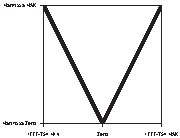
\includegraphics[page=1]{Number line.pdf}
\end{adjustbox}
\end{center}
\ppara{FIG.\hspace{0.2cm}\ref{fig:ieee_number_line} illustrates the IEEE-754 sign-magnitude representation, highlighting the fundamental discontinuity that occurs at zero.\hspace{0.2cm}The visualization shows how every numerical value has two distinct representations in the number space—positive and negative—that differ only by the sign bit, creating a mirrored duplicate of the entire number line.\hspace{0.2cm}This includes special cases like zero, which exists as both +0 and -0, despite representing the same mathematical value.\hspace{0.2cm}This sign-magnitude approach creates a discontinuity at zero and introduces significant branching complexity in numerical operations, requiring separate code paths for different sign combinations and explicit testing of the sign bit for most arithmetic operations.}
\newpage
\begin{lstlisting}[caption={SPIRIX Two's Complement Representation}, label={fig:spirix_number_line}]
\end{lstlisting}
\begin{center}
\begin{minipage}{0.48\textwidth}
  \centering
  \begin{adjustbox}{valign=t,width=\linewidth}
  \includegraphics[page=2]{Number line.pdf}
  \end{adjustbox}
\end{minipage}
\hfill
\begin{minipage}{0.48\textwidth}
  \centering
  \begin{adjustbox}{valign=t,width=\linewidth}
  \includegraphics[page=3]{Number line.pdf}
  \end{adjustbox}
\end{minipage}
\end{center}

\vspace{1cm}

\ppara{FIG.\hspace{0.2cm}\ref{fig:spirix_number_line}A presents a linear view of SPIRIX's continuous two's complement representation.\hspace{0.2cm}Unlike IEEE-754, SPIRIX achieves a completely continuous number space where values wrap around to maintain mathematical relationships across the entire range, eliminating the discontinuity at zero.\hspace{0.2cm}This continuity enables operations to cross the zero boundary without any special handling or branching.}

\ppara{FIG.\hspace{0.2cm}\ref{fig:spirix_number_line}B shows a vertically rotated perspective of the same representation, mapping values from fraction MAX/2+1 at the bottom to fraction MAX/2 at the top, with zero naturally landing in the middle.\hspace{0.2cm}This visualization highlights how zero is now a contiguous value in the number line rather than as a special case.}

\ppara{The sign can be determined by checking the most significant bit.\hspace{0.2cm}This representation enables a mathematically continuous space where values maintain their orientation/phase as they transition to exploded or vanished states.}
\newpage
\subsection*{Core Configuration Definitions}

\ppara{The Scalar and Circle configurations form the core of the SPIRIX system.\hspace{0.2cm}The following definitions outline their structure and representation:}

\begin{lstlisting}[style=rust, caption={Scalar Type Definition in Rust}, label={fig:scalar_structure}]
pub struct Scalar<F: Integer, E: Integer> {
	/// The normalized fraction component representing the significand.
	/// The fraction size determines the precision of the value.
	/// The N (prefix bit) pattern determines the number's state
	/// (normal, exploded, vanished, Zero or undefined/unimplemented).
	pub fraction: F,

	/// The exponent component determining the scale of the value/phase.
	/// The exponent size determines the range of the value/phase.
	/// When equal to AMBIGUOUS_EXPONENT, indicates an escaped phase
	/// (exploded, vanished, undefined/unimplemented or Zero).
	pub exponent: E,
}
\end{lstlisting}
\ppara{FIG.\hspace{0.2cm}\ref{fig:scalar_structure} presents the Rust implementation of the Scalar type, SPIRIX's representation for real numbers.\hspace{0.2cm}The structure shows the two primary components: a normalized two's complement fraction that determines precision, and an unbiased two's compliment exponent that determines range.\hspace{0.2cm}The type is parameterized to allow independent selection of fraction and exponent sizes according to application requirements.}
\newpage
\begin{lstlisting}[style=rust, caption={Circle Type Definition}, label={fig:circle_structure}]
pub struct Circle<F: Integer, E: Integer> {
	/// The real phase representing the real part of the complex number.
	/// The normalization level of this component indicates current state
	/// (normal, exploded, vanished, undefined/unimplemented, Zero).
	pub real: F,

	/// The imaginary component representing the phase of i.
	/// The normalization level of this component indicates current state
	/// (normal, exploded, vanished, undefined/unimplemented, Zero).
	pub imaginary: F,

	/// The shared exponent component determining the scale of both phases.
	/// When equal to AMBIGUOUS_EXPONENT, indicates an escaped phase
	/// (exploded, vanished, undefined or Zero).
	pub exponent: E,
}
\end{lstlisting}
\ppara{FIG.\hspace{0.2cm}\ref{fig:circle_structure} illustrates the Circle type definition for complex numbers in SPIRIX.\hspace{0.2cm}The structure contains real and imaginary fractions sharing a common exponent, enabling efficient complex arithmetic operations while maintaining mathematical consistency.\hspace{0.2cm}Like the Scalar, Circle is parameterized to allow customization of precision and range.}

\begin{lstlisting}[style=rust, caption={Where fraction: F and exponent: E are any sized integer}, label={fig:integer}]
impl Integer for i8 {}
impl Integer for i16 {}
impl Integer for i32 {}
impl Integer for i64 {}
impl Integer for i128 {}
\end{lstlisting}
\ppara{FIG.\hspace{0.2cm}\ref{fig:integer} demonstrates how SPIRIX abstracts over integer types.\hspace{0.2cm}While the implementation shown uses all of Rust's native signed integer sizes (i8 thru i128) for illustration, the system can work with any arbitrary-sized integers for both fraction and exponent components.\hspace{0.2cm}For example, custom integer sizes like <i12,i5> would be a perfectly valid implementation.\hspace{0.2cm}This flexibility enables applications to precisely tune configurations based on their specific precision and range requirements.}
\newpage
\begin{lstlisting}[caption={SPIRIX FE Type Configurations - Precision vs.\hspace{0.2cm}Range}, label={fig:spirix_configurations}]
\end{lstlisting}
\begin{table}[ht]
\centering
\renewcommand{\arraystretch}{1.5}
\begin{tabular}{|c|c|c|c|c|c|}
\hline
\multirow{2}{*}{\textbf{Range}} & \multicolumn{5}{c|}{\textbf{Precision (Fraction Bits)}} \\
\cline{2-6}
 & \textbf{F3} & \textbf{F4} & \textbf{F5} & \textbf{F6} & \textbf{F7} \\
 & \small{2.2 digits} & \small{4.6 digits} & \small{9.4 digits} & \small{19 digits} & \small{38.3 digits} \\
\hline
\textbf{E3} & F3E3 & F4E3 & F5E3 & F6E3 & F7E3 \\
\small{$\approx 10^{\pm2.1}$} & \small{$\langle$i8, i8$\rangle$} & \small{$\langle$i16, i8$\rangle$} & \small{$\langle$i32, i8$\rangle$} & \small{$\langle$i64, i8$\rangle$} & \small{$\langle$i128, i8$\rangle$} \\
\hline
\textbf{E4} & F3E4 & F4E4 & F5E4 & F6E4 & F7E4 \\
\small{$\approx 10^{\pm4.5}$} & \small{$\langle$i8, i16$\rangle$} & \small{$\langle$i16, i16$\rangle$} & \small{$\langle$i32, i16$\rangle$} & \small{$\langle$i64, i16$\rangle$} & \small{$\langle$i128, i16$\rangle$} \\
\hline
\textbf{E5} & F3E5 & F4E5 & F5E5 & F6E5 & F7E5 \\
\small{$\approx 10^{\pm9.3}$} & \small{$\langle$i8, i32$\rangle$} & \small{$\langle$i16, i32$\rangle$} & \small{$\langle$i32, i32$\rangle$} & \small{$\langle$i64, i32$\rangle$} & \small{$\langle$i128, i32$\rangle$} \\
\hline
\textbf{E6} & F3E6 & F4E6 & F5E6 & F6E6 & F7E6 \\
\small{$\approx 10^{\pm18.9}$} & \small{$\langle$i8, i64$\rangle$} & \small{$\langle$i16, i64$\rangle$} & \small{$\langle$i32, i64$\rangle$} & \small{$\langle$i64, i64$\rangle$} & \small{$\langle$i128, i64$\rangle$} \\
\hline
\textbf{E7} & F3E7 & F4E7 & F5E7 & F6E7 & F7E7 \\
\small{$\approx 10^{\pm38.2}$} & \small{$\langle$i8, i128$\rangle$} & \small{$\langle$i16, i128$\rangle$} & \small{$\langle$i32, i128$\rangle$} & \small{$\langle$i64, i128$\rangle$} & \small{$\langle$i128, i128$\rangle$} \\
\hline
\end{tabular}
\end{table}

\ppara{FIG.\hspace{0.2cm}\ref{fig:spirix_configurations} presents the matrix of valid SPIRIX FE type combinations, showing how precision (columns) and range (rows) can be independently configured.\hspace{0.2cm}The table provides approximate decimal digit precision and magnitude range for each configuration.}

\ppara{Scalar values are calculated as:}
\ppara{$value = fraction \times 2^{exponent}$}

\ppara{Circle values have real and imaginary phases sharing a common exponent:}
\ppara{$value = (real + imaginary \times i) \times 2^{exponent}$}

\newpage
\begin{lstlisting}[caption={SPIRIX Normalization Levels and Bit Patterns}, label={fig:normalization_levels}]
\end{lstlisting}
\begin{figure}[ht]
\centering
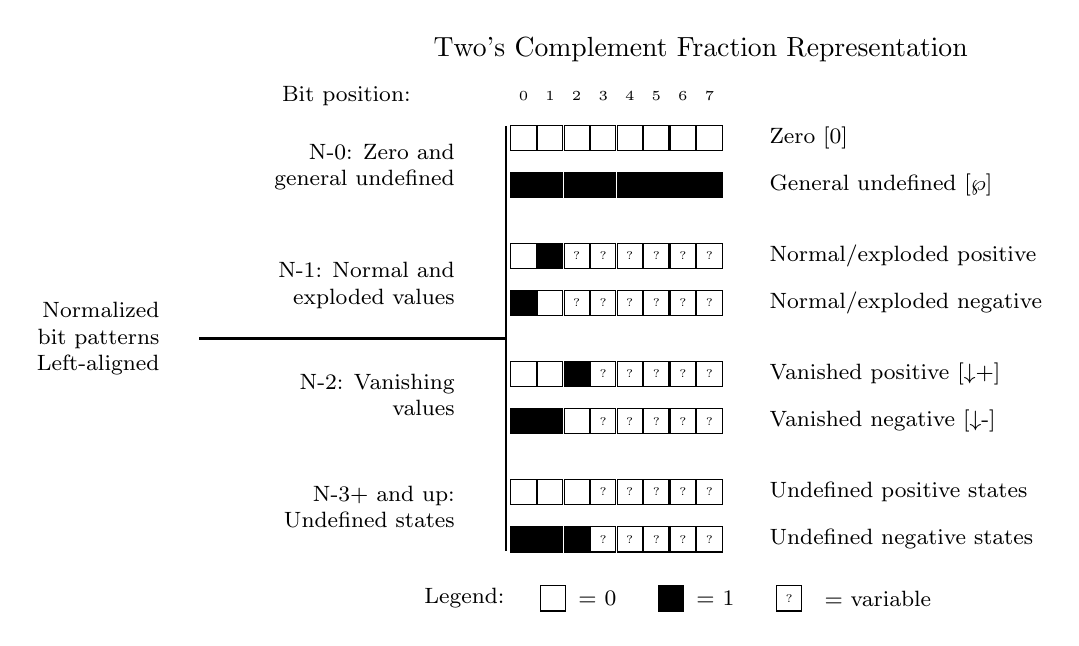
\begin{tikzpicture}[
    scale=0.75,
    every node/.style={font=\footnotesize},
    bit/.style={minimum width=0.4cm, minimum height=0.4cm, draw, anchor=center},
    highlight/.style={fill=black, text=white},
    empty/.style={fill=white},
    ]
    
    % Title
    \node at (4, 9.5) {\normalsize Two's Complement Fraction Representation};
    
    % Bit position markers
    \node[align=right] at (-2, 8.7) {Bit position:};
    \foreach \i in {0,...,7} {
        \node at (\i*0.45+1, 8.7) {\tiny \i};
    }
    
    % N-0: Zero and general undefined
    \node[align=right, anchor=east] at (0, 7.5) {N-0: Zero and\\general undefined};
    
    % Zero pattern
    \foreach \i in {0,...,7} {
        \node[bit, empty, scale=0.8] at (\i*0.45+1, 8) {};
    }
    \node[align=left, anchor=west] at (5, 8) {Zero [0]};
    
    % Undefined pattern
    \foreach \i in {0,...,7} {
        \node[bit, highlight, scale=0.8] at (\i*0.45+1, 7.2) {};
    }
    \node[align=left, anchor=west] at (5, 7.2) {General undefined [$\wp$]};
    
    % N-1: Normal and exploded values
    \node[align=right, anchor=east] at (0, 5.5) {N-1: Normal and\\exploded values};
    
    % Positive normal/exploded pattern
    \node[bit, empty, scale=0.8] at (1, 6) {};
    \node[bit, highlight, scale=0.8] at (1.45, 6) {};
    \foreach \i in {2,...,7} {
        \node[bit, scale=0.8] at (\i*0.45+1, 6) {\tiny?};
    }
    \node[align=left, anchor=west] at (5, 6) {Normal/exploded positive};
    
    % Negative normal/exploded pattern
    \node[bit, highlight, scale=0.8] at (1, 5.2) {};
    \node[bit, empty, scale=0.8] at (1.45, 5.2) {};
    \foreach \i in {2,...,7} {
        \node[bit, scale=0.8] at (\i*0.45+1, 5.2) {\tiny?};
    }
    \node[align=left, anchor=west] at (5, 5.2) {Normal/exploded negative};
    
    % N-2: Vanishing values
    \node[align=right, anchor=east] at (0, 3.65) {N-2: Vanishing\\values};
    
    % Positive vanished pattern
    \node[bit, empty, scale=0.8] at (1, 4) {};
    \node[bit, empty, scale=0.8] at (1.45, 4) {};
    \node[bit, highlight, scale=0.8] at (1.9, 4) {};
    \foreach \i in {3,...,7} {
        \node[bit, scale=0.8] at (\i*0.45+1, 4) {\tiny?};
    }
    \node[align=left, anchor=west] at (5, 4) {Vanished positive [$\downarrow$+]};
    
    % Negative vanished pattern
    \node[bit, highlight, scale=0.8] at (1, 3.2) {};
    \node[bit, highlight, scale=0.8] at (1.45, 3.2) {};
    \node[bit, empty, scale=0.8] at (1.9, 3.2) {};
    \foreach \i in {3,...,7} {
        \node[bit, scale=0.8] at (\i*0.45+1, 3.2) {\tiny?};
    }
    \node[align=left, anchor=west] at (5, 3.2) {Vanished negative [$\downarrow$-]};
    
    % N-3+: Specific undefined states
    \node[align=right, anchor=east] at (0, 1.75) {N-3+ and up:\\Undefined states};
    
    % Positive undefined patterns
    \node[bit, empty, scale=0.8] at (1, 2) {};
    \node[bit, empty, scale=0.8] at (1.45, 2) {};
    \node[bit, empty, scale=0.8] at (1.9, 2) {};
    \foreach \i in {3,...,7} {
        \node[bit, scale=0.8] at (\i*0.45+1, 2) {\tiny?};
    }
    \node[align=left, anchor=west] at (5, 2) {Undefined positive states};
    
    % Negative undefined patterns
    \node[bit, highlight, scale=0.8] at (1, 1.2) {};
    \node[bit, highlight, scale=0.8] at (1.45, 1.2) {};
    \node[bit, highlight, scale=0.8] at (1.9, 1.2) {};
    \foreach \i in {3,...,7} {
        \node[bit, scale=0.8] at (\i*0.45+1, 1.2) {\tiny?};
    }
    \node[align=left, anchor=west] at (5, 1.2) {Undefined negative states};
    
    \draw [thick] (0.7,8.2) -- (0.7,1);
    \draw [thick] (0.7,4.6) -- (-4.5,4.6);
    \node [align=right, anchor=east] at (-5, 4.6) {Normalized\\bit patterns\\Left-aligned};
    
    % Legend
    \node at (0, 0.2) {Legend:};
    \node[bit, empty, scale=0.8] at (1.5, 0.2) {};
    \node at (2.25, 0.2) {= 0};
    \node[bit, highlight, scale=0.8] at (3.5, 0.2) {};
    \node at (4.25, 0.2) {= 1};
    \node[bit, scale=0.8] at (5.5, 0.2) {\tiny?};
    \node at (7, 0.2) {= variable};
    
\end{tikzpicture}
\end{figure}

\ppara{FIG.\hspace{0.2cm}\ref{fig:normalization_levels} visualizes SPIRIX's left-aligned normalization scheme, showing how specific bit patterns in the most significant positions encode different numeric states.\hspace{0.2cm}The illustration demonstrates how normal values, exploded values, vanished values, and various undefined states are represented thru distinct bit patterns, where $\blacksquare$ represents binary 1s, $\square$ represents binary 0s, and $\hspace{0.35cm}$ represents variable bits holding numeric data.\hspace{0.2cm}This approach enables exponent only single check state detection without extensive branching, unlike IEEE-754 which requires explicit checking of exponent values and various fraction and sign bit combinations.\hspace{0.2cm}The normalization scheme supports any number of N-levels from N-0 up to the fraction bit size, allowing for future extension of states and capabilities as needed.\hspace{0.2cm}While the implementation shown here focuses on N-0 thru N-7 using 8-bit patterns for clarity, larger fraction sizes naturally accommodate additional normalization levels.\hspace{0.2cm}This extensibility ensures that the SPIRIX system can evolve to handle new mathematical implementations or domain-specific undefined states while maintaining backward compatibility with existing implementations.\hspace{0.2cm}The fraction component (or 'phase' in both Scalar and Circle types) follows this left-aligned normalized two's complement representation, while the exponent is stored as an unbiased two's complement integer with a single reserved value of one followed by all zeros (AMBIGUOUS\_EXPONENT) indicating non-normal states.\hspace{0.2cm}This reserved exponent serves as a consistent marker for all states outside normal representation, enabling efficient checking with a single exponent only comparison.\hspace{0.2cm}This unified approach drastically reduces the computational steps needed for most operations and greatly simplifies conversions between different precision and range configurations.}
\newpage
% \subsection*{Bit Patterns and Normalization Levels}

% \ppara{The SPIRIX system defines several N levels to represent numeric states:}

% \begin{lstlisting}[style=rust, caption={Bit Patterns for Numeric States}, label={fig:bit_patterns}]
% 01234567...\hspace{0.2cm}: Bit position

% N-0: Zero and general undefined/unimplemented
% ¡$\square\square\square\square\square\square\square\square$¡ Zero [0]
% ¡$\blacksquare\blacksquare\blacksquare\blacksquare\blacksquare\blacksquare\blacksquare\blacksquare$¡ General undefined [¡$\wp$¡]

% N-1: Normal and exploded Values approaching ¡$\infty$¡
% ¡$\square\blacksquare$¡xxxxxx | ¡$\blacksquare\square$¡xxxxxx  Normal [#,#] or exploded [¡$\uparrow$¡]
% (with AMBIGUOUS_EXPONENT)

% N-2: Vanishing values approaching Zero
% ¡$\square\square\blacksquare$¡xxxxx | ¡$\blacksquare\blacksquare\square$¡xxxxx Vanished [¡$\downarrow$¡]

% N-3+ and up: Specific undefined states
% ¡$\square\square\square$¡xxxxx | ¡$\blacksquare\blacksquare\blacksquare$¡xxxxx Various undefined states
% \end{lstlisting}
\subsection*{Undefined States}

\ppara{One of the key innovations in SPIRIX is the preservation of error information thru dedicated undefined patterns in the upper bits.\hspace{0.2cm}Unlike IEEE-754's single NaN value, SPIRIX uses specific bit patterns to track the cause of undefined operations:}

\begin{lstlisting}[style=rust, caption={Excerpt of Undefined State Definitions in Rust}, label={fig:undefined}]

/// ¡$\blacksquare\blacksquare\blacksquare\blacksquare\blacksquare\blacksquare\blacksquare\blacksquare$¡
pub const GENERAL: Undefined = Undefined {
	prefix: 0b11111111u8 as i8,
	symbol: "¡$\wp$¡",
	description: "General undefined",
};

// L3 Basic operators
/// ¡$\square\square\square\blacksquare\blacksquare\blacksquare\blacksquare\blacksquare$¡
pub const EXPLODED_PLUS_EXPLODED: Undefined = Undefined {
	prefix: 0b00011111u8 as i8,
	symbol: "¡$\wp$¡ ¡$\uparrow$¡+¡$\uparrow$¡",
	description: "Exploded value addition with exploded value",
};
/// ¡$\blacksquare\blacksquare\blacksquare\square\square\square\square\square$¡
pub const EXPLODED_MINUS_EXPLODED: Undefined = Undefined {
	prefix: 0b11100000u8 as i8,
	symbol: "¡$\wp$¡ ¡$\uparrow$¡-¡$\uparrow$¡",
	description: "Exploded value subtraction with exploded value",
};
/// ¡$\square\square\square\blacksquare\blacksquare\blacksquare\blacksquare\square$¡
pub const VANISHED_PLUS_VANISHED: Undefined = Undefined {
	prefix: 0b00011110u8 as i8,
	symbol: "¡$\wp$¡ ¡$\downarrow$¡+¡$\downarrow$¡",
	description: "Vanished value addition with vanished value",
};
/// ¡$\blacksquare\blacksquare\blacksquare\square\square\square\square\blacksquare$¡
pub const VANISHED_MINUS_VANISHED: Undefined = Undefined {
	prefix: 0b11100001u8 as i8,
	symbol: "¡$\wp$¡ ¡$\downarrow$¡-¡$\downarrow$¡",
	description: "Vanished value subtraction with vanished value",
};
// L4 Powers and roots
/// ¡$\square\square\square\square\blacksquare\blacksquare\blacksquare\blacksquare$¡
pub const EXPLODED_POWER: Undefined = Undefined {
	prefix: 0b00001111u8 as i8,
	symbol: "¡$\wp$¡ ¡$\uparrow$¡^",
	description: "Exploded value raised to power",
};
/// ¡$\blacksquare\blacksquare\blacksquare\blacksquare\square\square\square\square$¡
pub const VANISHED_POWER: Undefined = Undefined {
	prefix: 0b11110000u8 as i8,
	symbol: "¡$\wp$¡ ¡$\downarrow$¡^",
	description: "Vanished value raised to power",
};
/// ¡$\square\square\square\square\blacksquare\blacksquare\blacksquare\square$¡
pub const POWER_EXPLODED: Undefined = Undefined {
	prefix: 0b00001110u8 as i8,
	symbol: "¡$\wp$¡ ^¡$\uparrow$¡",
	description: "Value raised to exploded power",
};

// L5 Logarithms
/// ¡$\square\square\square\square\square\blacksquare\blacksquare\blacksquare$¡
pub const EXPLODED_LOG: Undefined = Undefined {
	prefix: 0b00000111u8 as i8,
	symbol: "¡$\wp$¡ ¡$\uparrow$¡@",
	description: "Logarithm of exploded value",
};
/// ¡$\blacksquare\blacksquare\blacksquare\blacksquare\blacksquare\square\square\square$¡
pub const VANISHED_LOG: Undefined = Undefined {
	prefix: 0b11111000u8 as i8,
	symbol: "¡$\wp$¡ ¡$\downarrow$¡@",
	description: "Logarithm of vanished value",
};
/// ¡$\square\square\square\square\square\blacksquare\blacksquare\square$¡
pub const LOG_EXPLODED: Undefined = Undefined {
	prefix: 0b00000110u8 as i8,
	symbol: "¡$\wp$¡ @¡$\uparrow$¡",
	description: "Logarithm with exploded base",
};

// L6 Sine/Cosine
/// ¡$\square\square\square\square\square\square\blacksquare\blacksquare$¡
pub const SINE: Undefined = Undefined {
	prefix: 0b00000011u8 as i8,
	symbol: "¡$\wp$¡ s",
	description: "Sine of value with imprecise period position",
};
/// ¡$\blacksquare\blacksquare\blacksquare\blacksquare\blacksquare\blacksquare\square\square$¡
pub const COSINE: Undefined = Undefined {
	prefix: 0b11111100u8 as i8,
	symbol: "¡$\wp$¡ c",
	description: "Cosine of value with imprecise period position",
};

// L7 Tangent and extensions
/// ¡$\square\square\square\square\square\square\square\blacksquare$¡
pub const TANGENT: Undefined = Undefined {
	prefix: 0b00000001u8 as i8,
	symbol: "¡$\wp$¡ t",
	description: "Tangent of value with imprecise period position",
};
/// ¡$\blacksquare\blacksquare\blacksquare\blacksquare\blacksquare\blacksquare\blacksquare\square$¡
pub const EXTENDED_UNDEFINED: Undefined = Undefined {
	prefix: 0b11111110u8 as i8,
	symbol: "¡$\wp$¡",
	description: "Reserved for undefined extensions",
};
\end{lstlisting}

\ppara{FIG.\hspace{0.2cm}\ref{fig:undefined} illustrates SPIRIX's hierarchy of undefined states.\hspace{0.2cm}Unlike IEEE-754's single NaN representation, SPIRIX employs specific bit patterns to encode the precise cause of undefined operations.\hspace{0.2cm}The figure shows how each undefined state is defined with a unique prefix, a symbol (like "℘ $\uparrow$+$\uparrow$"), and a descriptive name.\hspace{0.2cm}The system preserves the first cause of undefined operations during propagation, for example when computing "0$\^{}$0 + 1/0 = ℘0$\^{}$0" maintains the initial undefined cause (Zero raised to Zero power) thruout subsequent operations.\hspace{0.2cm}By assigning different undefined operations with unique states, SPIRIX enables precise error tracking, allowing users to trace numerical issues to their origin rather than encountering a generic "Not a Number" error.}
\newpage
\subsection*{IEEE-754 Numerical Operations}
\ppara{In IEEE-754, floating-point operations follow a complex sequence of steps with numerous special case handling requirements.\hspace{0.2cm}The sign-magnitude representation necessitates explicit sign bit testing for virtually all operations.\hspace{0.2cm}For basic arithmetic functions like addition and subtraction, the processor must first examine sign bits to determine whether to perform addition or subtraction of magnitudes, followed by potential sign adjustment of the result.\hspace{0.2cm}This sign-dependent processing path creates a fundamental bifurcation in the execution flow.}
\ppara{Multiplication and division operations in IEEE-754 similarly require sign bit extraction and separate processing.\hspace{0.2cm}The sign of the result is determined by XORing the sign bits of operands, while magnitude calculations proceed independently.\hspace{0.2cm}Special values like NaN, infinities, zeros (both positive and negative), and subnormal numbers each trigger distinct processing paths with their own rules and exceptions.\hspace{0.2cm}For example, multiplication between zero and infinity produces NaN, while division of a finite non-zero value by zero produces either positive or negative infinity depending on operand signs.}
\ppara{Transcendental functions in IEEE-754 contain extensive special case handling for boundary values.\hspace{0.2cm}Functions like logarithm, sine, and tangent must implement separate processing for inputs near zero, extremely large values, negative numbers, and special values.\hspace{0.2cm}Each of these cases introduces additional branching, often requiring multiple comparison operations and conditional jumps that impact instruction pipeline efficiency and predictability.\hspace{0.2cm}This branching complexity becomes particularly problematic in SIMD (Single Instruction Multiple Data) processing environments, where divergent execution paths across data lanes can significantly degrade performance thru serialization of what should be parallel operations.}
\ppara{The subtraction operation in IEEE-754 exemplifies the implementation challenges inherent in the standard's approach.\hspace{0.2cm}Subtraction requires careful examination of sign combinations to determine whether to perform a true subtraction or convert to addition with sign inversion.\hspace{0.2cm}This operation-specific branching adds considerable complexity to hardware implementations and compiler optimization efforts, making efficient pipelining difficult to achieve.}
\newpage
\begin{lstlisting}[caption={IEEE-754 Subtraction Flowchart}, label={fig:ieee_subtract_flowchart}]
\end{lstlisting}
\begin{figure}[htbp]
  \centering
  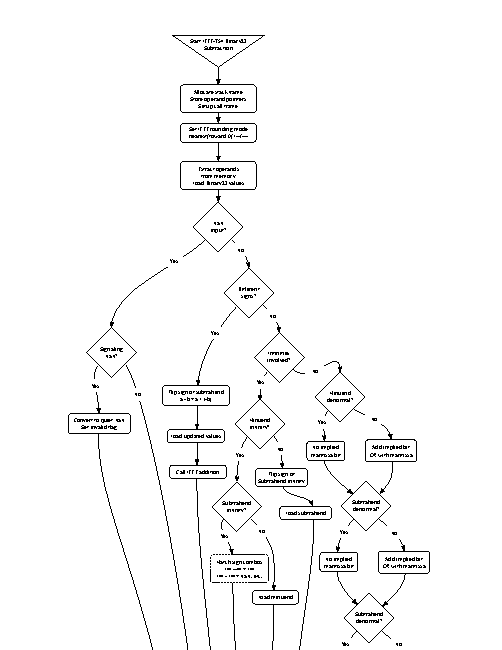
\includepdf[pages=1, scale=0.85]{IEEE subtract flowchart.pdf}
\end{figure}
\newpage
\begin{figure}[htbp]
  \centering
  \includepdf[pages=2, scale=0.85]{IEEE subtract flowchart.pdf}
\end{figure}
\newpage
\begin{figure}[htbp]
  \centering
  \includepdf[pages=3, scale=0.85]{IEEE subtract flowchart.pdf}
\end{figure}
\newpage
% \begin{lstlisting}[caption={Subtraction Operation Complexity: IEEE-754 Subtraction}, label={fig:ieee_subtract_flowchart}]
% \end{lstlisting}
% \begin{figure}[ht]
% \centering
% \begin{tikzpicture}[
%     scale=1,
%     every node/.style={font=\small},
%     process/.style={rectangle, draw, minimum width=3cm, minimum height=0.7cm, align=center},
%     decision/.style={diamond, draw, minimum width=2.5cm, minimum height=1cm, text centered, align=center},
%     arrow/.style={->, >=Stealth, thick},
%     complex/.style={rectangle, rounded corners, draw, fill=red!10, minimum width=3cm, minimum height=0.7cm, align=center},
%     ]
    
%     % Title
%     \node at (8, 11) {\Large Subtraction Operation Complexity: IEEE-754 vs.\hspace{0.2cm}SPIRIX};
    
%     % IEEE-754 side
%     \node at (4, 10) {\textbf{IEEE-754 Binary32 Subtraction}};
    
%     % Starting node
%     \node[process] (ieee_start) at (4, 9) {Start IEEE-754 Subtraction};
    
%     % Special value checks
%     \node[decision] (ieee_special) at (4, 7.5) {Special\\values?};
%     \node[complex] (ieee_nan) at (1, 6) {NaN handling\\(multiple cases)};
%     \node[complex] (ieee_inf) at (4, 6) {Infinity handling\\(multiple cases)};
%     \node[complex] (ieee_zero) at (7, 6) {Zero handling\\(multiple cases)};
    
%     % Sign handling
%     \node[decision] (ieee_sign) at (4, 4.5) {Same\\signs?};
    
%     % Different sign paths
%     \node[complex] (ieee_diff_sign) at (1, 3) {Convert to addition\\change sign};
    
%     % Same sign path
%     \node[decision] (ieee_exp) at (7, 3) {Equal\\exponents?};
    
%     % Exponent paths
%     \node[complex] (ieee_align) at (5, 1.5) {Align mantissas\\(shift smaller)};
%     \node[process] (ieee_sub) at (9, 1.5) {Subtract mantissas};
    
%     % Normalization
%     \node[complex] (ieee_norm) at (7, 0) {Normalize result\\(multiple cases)};
    
%     % Result
%     \node[process] (ieee_result) at (4, -1.5) {Return IEEE-754 result};
    
%     % Arrows
%     \draw[arrow] (ieee_start) -- (ieee_special);
%     \draw[arrow] (ieee_special) -- node[left] {Yes} (ieee_nan);
%     \draw[arrow] (ieee_special) -- (ieee_inf);
%     \draw[arrow] (ieee_special) -- node[right] {Zeros} (ieee_zero);
%     \draw[arrow] (ieee_special) -- node[right] {No} (ieee_sign);
    
%     \draw[arrow] (ieee_nan) |- (ieee_result);
%     \draw[arrow] (ieee_inf) |- (ieee_result);
%     \draw[arrow] (ieee_zero) |- (ieee_result);
    
%     \draw[arrow] (ieee_sign) -- node[left] {No} (ieee_diff_sign);
%     \draw[arrow] (ieee_sign) -- node[right] {Yes} (ieee_exp);
    
%     \draw[arrow] (ieee_diff_sign) |- (ieee_result);
    
%     \draw[arrow] (ieee_exp) -- node[left] {No} (ieee_align);
%     \draw[arrow] (ieee_exp) -- node[right] {Yes} (ieee_sub);
    
%     \draw[arrow] (ieee_align) -- (ieee_sub);
%     \draw[arrow] (ieee_sub) -- (ieee_norm);
%     \draw[arrow] (ieee_norm) -- (ieee_result);
    
%     % SPIRIX side
%     \node at (14, 10) {\textbf{SPIRIX Scalar Subtraction}};
    
%     % Starting node
%     \node[process] (spirix_start) at (14, 9) {Start SPIRIX Subtraction};
    
%     % Check for normal values
%     \node[decision] (spirix_normal) at (14, 7.5) {Both\\normal?};
    
%     % Handle ambiguous cases
%     \node[process] (spirix_ambig) at (17, 6) {Handle ambiguous cases};
    
%     % Process normal values
%     \node[process] (spirix_comp) at (11, 6) {Compare exponents};
    
%     % Align fractions
%     \node[process] (spirix_align) at (11, 4.5) {Align fractions by\\exponent difference};
    
%     % Subtract
%     \node[process] (spirix_sub) at (11, 3) {Perform two's complement\\subtraction};
    
%     % Normalize
%     \node[process] (spirix_norm) at (11, 1.5) {Normalize result\\using leading bits};
    
%     % Check underflow
%     \node[process] (spirix_under) at (11, 0) {Check for\\underflow};
    
%     % Handle special cases
%     \node[process] (spirix_spec1) at (17, 4.5) {Return if either\\is undefined};
%     \node[process] (spirix_spec2) at (17, 3) {Handle exploded\\combinations};
%     \node[process] (spirix_spec3) at (17, 1.5) {Handle vanished\\combinations};
%     \node[process] (spirix_spec4) at (17, 0) {Handle Zero\\combinations};
    
%     % Result
%     \node[process] (spirix_result) at (14, -1.5) {Return normalized SPIRIX result};
    
%     % Arrows
%     \draw[arrow] (spirix_start) -- (spirix_normal);
%     \draw[arrow] (spirix_normal) -- node[left] {Yes} (spirix_comp);
%     \draw[arrow] (spirix_normal) -- node[right] {No} (spirix_ambig);
    
%     \draw[arrow] (spirix_comp) -- (spirix_align);
%     \draw[arrow] (spirix_align) -- (spirix_sub);
%     \draw[arrow] (spirix_sub) -- (spirix_norm);
%     \draw[arrow] (spirix_norm) -- (spirix_under);
%     \draw[arrow] (spirix_under) -- (spirix_result);
    
%     \draw[arrow] (spirix_ambig) -- (spirix_spec1);
%     \draw[arrow] (spirix_spec1) -- (spirix_spec2);
%     \draw[arrow] (spirix_spec2) -- (spirix_spec3);
%     \draw[arrow] (spirix_spec3) -- (spirix_spec4);
%     \draw[arrow] (spirix_spec4) -- (spirix_result);
    
%     % Comparison annotations
%     \node[draw, fill=red!10, text width=4cm, align=center] at (4, -3) {
%         Multiple branching paths\\
%         Sign-dependent logic\\
%         Special case explosion
%     };
    
%     \node[draw, fill=green!10, text width=4cm, align=center] at (14, -3) {
%         Two main paths only\\
%         Sign-agnostic processing\\
%         Uniform special case handling
%     };
    
%     % Draw dividing line
%     \draw[dashed] (8.5,-3.5) -- (8.5,11.5);
    
% \end{tikzpicture}
% \end{figure} % Claude!!! This will get replaced with those pdf pages as the illustration got nasty and I had to do it in illustrator

\ppara{FIG.\hspace{0.2cm}\ref{fig:ieee_subtract_flowchart} details the elaborate control flow required for IEEE-754 subtraction operations.\hspace{0.2cm}The flowchart reveals numerous branching paths needed to handle different sign combinations, exponent comparisons, and special value cases, illustrating the implementation complexity that results from IEEE-754's disjoint representation of signs and fractions.}


\subsection*{Spirix Numerical Operations}
\ppara{In contrast, the SPIRIX implementation maintains a streamlined approach with only two main execution paths: one for normal values and one for ambiguous cases.\hspace{0.2cm}This simplification eliminates the need for sign-specific logic and special case explosion, resulting in more predictable execution paths and improved performance, especially in SIMD environments.}

\subsection*{Scalar Subtraction Implementation}

\ppara{This section demonstrates subtraction as an example of how SPIRIX handles arithmetic operations.}
% \begin{lstlisting}[caption={Scalar Subtraction Flowchart}, label={fig:scalar_subtract_flowchart}]
% \end{lstlisting}
% \fbox{
% \begin{minipage}{\textwidth}
% \begin{figure}[H]
% \centering
% \begin{tikzpicture}[
%     node distance=1cm,
%     startstop/.style={rectangle, rounded corners, minimum width=3cm, minimum height=0.8cm, text centered, draw=black, font=\small},
%     process/.style={rectangle, minimum width=3cm, minimum height=0.8cm, text centered, draw=black, font=\small, align=center},
%     decision/.style={diamond, minimum width=2.5cm, minimum height=1cm, text centered, draw=black, font=\small, align=center},
%     arrow/.style={thick,->,>=stealth}
% ]

% % Start
% \node (start) [startstop] {Start Scalar Subtraction};

% % Check for normal values
% \node (normal-check) [decision, below=of start] {Both\\ normal?};

% % === Main path ===
% \node (exponent-compare) [process, below left=1.5cm and 0.8cm of normal-check] {Compare exponents};

% \node (main-path) [process, below=of exponent-compare] {Align fractions by\\ exponent difference};
% \node (perform-subtraction) [process, below=of main-path] {Perform two's\\ complement subtraction};
% \node (normalize) [process, below=of perform-subtraction] {Normalize result\\ using leading bits};
% \node (adjust-exponent) [process, below=of normalize] {Subtract shift\\ from exponent};
% \node (check-underflow) [process, below=of adjust-exponent] {Check for underflow\\ overflow is naturally handled};
% \node (return1) [startstop, below=of check-underflow] {Return normalized result};

% % === Ambiguous cases - right branch ===
% \node (ambiguous-cases) [process, below right=1.5cm and 0.8cm of normal-check] {Handle ambiguous cases};

% % Ambiguous case checks as a sequence
% \node (undefined) [process, below=of ambiguous-cases] {Return if either\\ is undefined};
% \node (exploded-cases) [process, below=of undefined] {Handle exploded\\ value combinations};
% \node (vanished-cases) [process, below=of exploded-cases] {Handle vanished\\ value combinations};
% \node (zero-cases) [process, below=of vanished-cases] {Handle zero\\ combinations};
% \node (return3) [startstop, below=of zero-cases] {Return appropriate result};

% % Connect nodes with arrows
% \draw [arrow] (start) -- (normal-check);
% \draw [arrow] (normal-check) -- node[above left, font=\scriptsize] {Yes} (exponent-compare);
% \draw [arrow] (normal-check) -- node[above right, font=\scriptsize] {No} (ambiguous-cases);

% \draw [arrow] (exponent-compare) -- (main-path);
% \draw [arrow] (main-path) -- (perform-subtraction);
% \draw [arrow] (perform-subtraction) -- (normalize);
% \draw [arrow] (normalize) -- (adjust-exponent);
% \draw [arrow] (adjust-exponent) -- (check-underflow);
% \draw [arrow] (check-underflow) -- (return1);

% \draw [arrow] (ambiguous-cases) -- (undefined);
% \draw [arrow] (undefined) -- (exploded-cases);
% \draw [arrow] (exploded-cases) -- (vanished-cases);
% \draw [arrow] (vanished-cases) -- (zero-cases);
% \draw [arrow] (zero-cases) -- (return3);

% \end{tikzpicture}
% \end{figure}
% \vspace{0.5cm}
% \end{minipage}
% }
\newpage
\begin{lstlisting}[caption={Scalar Subtraction Flowchart}, label={fig:scalar_subtract_flowchart}]
\end{lstlisting}
\begin{figure}[htbp]
  \centering
  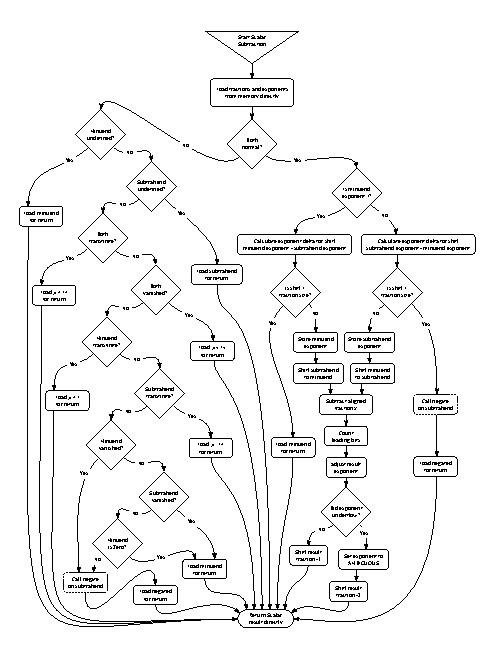
\includepdf[pages=1, scale=0.85]{Scalar subtract flowchart.pdf}
\end{figure}
\newpage

\ppara{FIG.\hspace{0.2cm}\ref{fig:scalar_subtract_flowchart} illustrates the streamlined control flow of SPIRIX scalar subtraction.\hspace{0.2cm}The diagram shows just two primary paths: one for normal values and one for ambiguous cases, with minimal branching in each path.\hspace{0.2cm}This simpler structure directly results from SPIRIX's continuous two's complement representation, which eliminates the need for special sign handling and separate magnitudes.}
\ppara{A key innovation in Spirix is how overflow handling occurs naturally thru the numeric structure itself.\hspace{0.2cm}During normalization, an exponent exceeding maximum wraps to the AMBIGUOUS\_EXPONENT value, indicating an exploded state without any conditional checks or operations.\hspace{0.2cm}Additionally, the memory-aligned fraction and exponent sizes eliminate bit packing operations, allowing results to be returned directly.}

\subsection*{IEEE-754 Binary32 Subtraction Implementation}

\begin{lstlisting}[style=rust, caption={Annotated Binary32 Normal Case Subtraction Instruction Trace}, label={fig:ieee_subtract}]
; Main Subtraction Fuction Entry Point
[001]sub rsp, 0x58                 ; Allocate 88 bytes on the stack
[002]mov qword ptr [rsp 0x8], rdi  ; Store first parameter (pointer to first value)
[003]mov al, dl                    ; Move the 3rd parameter (lower byte) to al
[004]mov dword ptr [rsp 0x18], esi ; Store second parameter (second value)
[005]mov ecx, dword ptr [rsp 0x18] ; Load second Binary32 value into ecx
[006]mov dword ptr [rsp 0x14], ecx ; Store second Binary32 value at rsp+20
[007]mov byte ptr [rsp 0x1f], al   ; Store lower byte of 3rd parameter at rsp+31
[008]mov qword ptr [rsp 0x30], rdi ; Move first parameter
[009]lea rax, ptr [rip 0x3d6e9]    ; Load effective address
[010]lea rdi, ptr [rsp 0x1f]       ; Load address of next function into rdi
[011]call rax                      ; Call function at address in rax

; Set Rounding Mode
[012]push rax                 ; Save rax register
[013]mov qword ptr [rsp], rdi ; Store rdi at top of stack
[014]call 0x558bdf671e20      ; Call function to set rounding mode

; Convert Rounding Mode to Float Format
[015]mov qword ptr [rsp-0x8], rdi      ; Store rdi at rsp-8
[016]movzx eax, byte ptr [rdi]         ; Zero-extend byte at [rdi] into eax
[017]mov qword ptr [rsp-0x18], rax     ; Store extended value at rsp-24
[018]mov rax, qword ptr [rsp-0x18]     ; Load value from rsp-24 into rax
[019]lea rcx, ptr [rip 0x452af]        ; Load effective address (jump table?)
[020]movsxd rax, dword ptr [rcx rax*4] ; Load and sign-extend value from jump table
[021]add rax, rcx                      ; Add base address to jump offset
[022]jmp rax                           ; Jump to the calculated address
[023]mov byte ptr [rsp-0x9], 0x0       ; Set byte at rsp-9 to 0
[024]jmp 0x558bdf671e65                ; Jump to function epilogue
[025]mov al, byte ptr [rsp-0x9]        ; Load byte from rsp-9 into al
[026]ret                               ; Return from function

; Set Rounding Mode
[027]movzx edi, al                ; Zero-extend al into edi
[028]call qword ptr [rip 0x5bf45] ; Call function pointer at rip+0x5bf45

; Rounding Mode Helper
[029]push rbp                     ; Save base pointer
[030]mov rbp, rsp                 ; Set new base pointer
[031]push rbx                     ; Save rbx register
[032]sub rsp, 0x8                 ; Allocate 8 bytes on stack
[033]mov ebx, edi                 ; Store first parameter in ebx
[034]mov rax, qword ptr fs:[0x0]  ; Load value from fs segment
[035]lea rax, ptr [rax-0x4f]      ; Calculate address at fs:0 - 79
[036]mov byte ptr [rax], bl       ; Store lowest byte of ebx at calculated address
[037]mov rbx, qword ptr [rbp-0x8] ; Restore rbx
[038]leave                        ; Restore stack and base pointer
[039]ret                          ; Return from function

; Set Rounding Mode (continued)
[040]pop rax ; Restore rax
[041]ret     ; Return from function

; Main Subtraction Function (continued)
[042]jmp 0x558bdf63473a            ; Jump to next part of subtraction function
[043]mov rax, qword ptr [rsp 0x8]  ; Load pointer to first Binary32 from rsp+8
[044]mov eax, dword ptr [rax]      ; Load value of first Binary32 into eax
[045]mov dword ptr [rsp 0x28], eax ; Store first Binary32 at rsp+40
[046]lea rdi, ptr [rsp 0x14]       ; Load address of second value into rdi
[047]call 0x558bdf6346e0           ; Call function to borrow memory value

; Borrow Memory Value
[048]mov rax, rdi                 ; Copy input parameter to rax
[049]mov qword ptr [rsp-0x8], rax ; Store rax at rsp-8
[050]ret                          ; Return from function

; Main Subtraction Function (continued)
[051]mov qword ptr [rsp], rax      ; Store return value at top of stack
[052]jmp 0x558bdf634755            ; Jump to next part of subtraction
[053]mov rax, qword ptr [rsp]      ; Load pointer from stack into rax
[054]mov eax, dword ptr [rax]      ; Load value at pointer into eax
[055]mov dword ptr [rsp 0x2c], eax ; Store second Binary32 at rsp+44
[056]mov eax, dword ptr [rsp 0x28] ; Load first Binary32 into eax
[057]mov dword ptr [rsp 0x4c], eax ; Store first Binary32 at rsp+76
[058]mov edi, dword ptr [rsp 0x4c] ; Load first value into edi
[059]mov eax, dword ptr [rsp 0x2c] ; Load second Binary32 into eax
[060]mov dword ptr [rsp 0x50], eax ; Store second Binary32 at rsp+80
[061]mov esi, dword ptr [rsp 0x50] ; Load second value into esi
[062]call qword ptr [rip 0x9906b]  ; Call function for low-level

; Low-level Float Subtraction
[063]push rbp            ; Save base pointer
[064]mov rbp, rsp        ; Set new base pointer
[065]mov eax, edi        ; Copy first Binary32 to eax
[066]mov edx, esi        ; Copy second Binary32 to edx
[067]xor esi, edi        ; XOR the two Binary32 values
[068]js 0x558bdf671e83   ; Jump if sign bit is set (opposing signs)
[069]mov rsi, rdx        ; Copy second Binary32 to rsi
[070]mov rdi, rax        ; Copy first Binary32 to rdi
[071]call 0x558bdf6721a9 ; Call function to add float magnitudes

; Add Float Magnitudes
[072]push rbp            ; Save base pointer
[073]mov rbp, rsp        ; Set new base pointer
[074]mov rcx, rdi        ; Copy first Binary32 to rcx
[075]shr rcx, 0x17       ; Shift right by 23 bits (extract exponent)
[076]movzx ecx, cl       ; Zero-extend lowest byte to get 8-bit exponent
[077]mov r9, rcx         ; Copy exponent to r9
[078]mov r10, rdi        ; Copy first Binary32 to r10
[079]and r10d, 0x7fffff  ; Mask to get mantissa (23 bits)
[080]mov rax, rsi        ; Copy second Binary32 to rax
[081]shr rax, 0x17       ; Shift right by 23 bits (extract exponent)
[082]movzx eax, al       ; Zero-extend lowest byte to get 8-bit exponent
[083]mov rdx, rsi        ; Copy second Binary32 to rdx
[084]and edx, 0x7fffff   ; Mask to get mantissa (23 bits)
[085]mov r11, rcx        ; Copy first exponent to r11
[086]sub r11, rax        ; Subtract exponents (for comparing magnitude)
[087]jnz 0x558bdf67224f  ; Jump if exponents are different
[088]mov r8d, edi        ; Copy first Binary32 to r8d
[089]shr r8d, 0x1f       ; Shift right by 31 bits (extract sign bit)
[090]shl r10, 0x6        ; Shift first mantissa left by 6 bits (normalize)
[091]shl rdx, 0x6        ; Shift second mantissa left by 6 bits (normalize)
[092]test r11, r11       ; Test if exponent difference is Zero
[093]js 0x558bdf6722c4   ; Jump if exponent difference is negative
[094]cmp rax, 0xff       ; Check for NaN/Infinity
[095]jz 0x558bdf67230b   ; Jump if second number is NaN or Infinity
[096]test rcx, rcx       ; Test if first exponent is Zero
[097]mov esi, 0x20000000 ; Set esi to 0x20000000 (implied 1 for normal numbers)
[098]cmovz rsi, r10      ; True for normals, false for subnormal
[099]mov rdi, rax        ; Copy second exponent to rdi
[100]sub rdi, rcx        ; Calculate exponent difference
[101]add rsi, r10        ; Add implied 1 to first mantissa
[102]cmp rdi, 0x1e       ; Compare exponent difference with 30
[103]jnbe 0x558bdf672327 ; Jump if difference is not within range
[104]mov ecx, edi        ; Copy exponent difference to ecx
[105]neg ecx             ; Negate exponent difference
[106]mov r9d, esi        ; Copy first mantissa with implied 1 to r9d
[107]shl r9d, cl         ; Shift left by exponent difference
[108]test r9d, r9d       ; Test if shifted value is Zero
[109]setnz r10b          ; Set r10b to 1 if not Zero, 0 if Zero
[110]movzx r10d, r10b    ; Zero-extend r10b to r10d
[111]mov ecx, edi        ; Copy exponent difference to ecx
[112]shr esi, cl         ; Shift first mantissa right by exponent difference
[113]or r10d, esi        ; Combine shifted bits with sticky bit
[114]mov r10d, r10d      ; Clear upper 32 bits of r10
[115]mov r9, rax         ; Copy second exponent to r9
[116]jmp 0x558bdf6722a3  ; Jump to next part of float addition
[117]lea rdx, ptr [r10 rdx*1 0x20000000] ; Calculate sum of mantissas
[118]cmp rdx, 0x3fffffff ; Check if result needs normalization
[119]jnbe 0x558bdf67220e ; Jump if normalization needed
[120]movzx edi, r8b      ; Zero-extend sign bit to edi
[121]mov rsi, r9         ; Copy exponent to rsi
[122]call 0x558bdf671f65 ; Call function to round and pack to Binary32 format

; Round and Pack to Binary32 Format
[123]push rbp                      ; Save base pointer
[124]mov rbp, rsp                  ; Set new base pointer
[125]push r15                      ; Save r15 register
[126]push r14                      ; Save r14 register
[127]push r13                      ; Save r13 register
[128]push r12                      ; Save r12 register
[129]push rbx                      ; Save rbx register
[130]sub rsp, 0x18                 ; Allocate 24 bytes on stack
[131]mov r15d, edi                 ; Store sign bit in r15d
[132]mov dword ptr [rbp-0x34], edi ; Store sign bit at rbp-52
[133]mov rbx, rsi                  ; Store exponent in rbx
[134]mov r13, rdx                  ; Store mantissa in r13
[135]mov rax, qword ptr fs:[0x0]   ; Load value from fs segment
[136]lea rax, ptr [rax-0x4f]       ; Calculate address at fs:0 - 79
[137]movzx r14d, byte ptr [rax]    ; Load rounding mode into r14d
[138]test r14b, r14b               ; Test if rounding mode is 0 (to nearest)
[139]setz byte ptr [rbp-0x40]      ; Set flag at rbp-64 if rounding mode is 0
[140]mov r12d, 0x40                ; Set r12d to 64 (used for rounding)
[141]test r14b, 0xfb               ; Test rounding mode against 0xfb
[142]jz 0x558bdf671fc9             ; Jump if specific rounding mode
[143]mov r15d, r13d                ; Copy mantissa to r15d
[144]and r15d, 0x7f                ; Mask with 0x7f (7 least significant bits)
[145]mov dword ptr [rbp-0x38], ebx ; Store exponent at rbp-56
[146]cmp ebx, 0xfc                 ; Compare exponent with 0xfc
[147]jbe 0x558bdf672000            ; Jump if exponent <= 0xfc
[148]movzx r12d, r12b              ; Zero-extend r12b to r12d
[149]add r12, r13                  ; Add mantissa to r12
[150]shr r12, 0x7                  ; Shift right by 7 bits (rounding)
[151]test r15b, r15b               ; Test if lower 7 bits are Zero
[152]jnz 0x558bdf6720ec            ; Jump if lower 7 bits are not Zero
[153]mov rax, qword ptr fs:[0x0]   ; Load value from fs segment
[154]lea rax, ptr [rax-0x50]       ; Calculate address at fs:0 - 80
[155]or byte ptr [rax], 0x1        ; Set inexact flag
[156]cmp r14b, 0x6                 ; Compare rounding mode with 6
[157]jnz 0x558bdf672014            ; Jump if rounding mode is not 6
[158]cmp r15b, 0x40                ; Compare lower 7 bits with 0x40
[159]setz al                       ; Set al to 1 if equal, 0 if not
[160]movzx eax, al                 ; Zero-extend al to eax
[161]and rax, qword ptr [rbp-0x40] ; AND with rounding flag
[162]not rax                       ; Complement result
[163]and r12, rax                  ; Mask r12 with result
[164]mov eax, 0x0                  ; Set eax to 0
[165]cmovz rbx, rax                ; If Zero, set exponent to 0
[166]mov eax, dword ptr [rbp-0x34] ; Load sign bit into eax
[167]shl eax, 0x1f                 ; Shift sign bit to position 31
[168]shl ebx, 0x17                 ; Shift exponent to position 23-30
[169]add eax, ebx                  ; Combine sign and exponent
[170]mov eax, eax                  ; Clear upper 32 bits
[171]add rax, r12                  ; Add mantissa to result
[172]add rsp, 0x18                 ; Deallocate stack space
[173]pop rbx                       ; Restore rbx
[174]pop r12                       ; Restore r12
[175]pop r13                       ; Restore r13
[176]pop r14                       ; Restore r14
[177]pop r15                       ; Restore r15
[178]pop rbp                       ; Restore base pointer
[179]ret                           ; Return from function

; Add Float Magnitudes (epilogue)
[180]pop rbp ; Restore base pointer
[181]ret     ; Return from function

; Low-level Float Subtraction (epilogue)
[182]jmp 0x558bdf671e81 ; Jump to another part of function
[183]pop rbp            ; Restore base pointer
[184]ret                ; Return from function

; Main Subtraction Function (epilogue)
[185]mov dword ptr [rsp 0x54], eax ; Store result at rsp+84
[186]mov eax, dword ptr [rsp 0x54] ; Load result back into eax
[187]mov dword ptr [rsp 0x24], eax ; Store result at rsp+36
[188]mov eax, dword ptr [rsp 0x24] ; Load result back into eax
[189]mov dword ptr [rsp 0x20], eax ; Store result at rsp+32
[190]mov eax, dword ptr [rsp 0x20] ; Load result back into eax
[191]add rsp, 0x58                 ; Deallocate 88 bytes from stack
[192]ret                           ; Return from function

\end{lstlisting}

\ppara{The IEEE-754 subtraction implementation shown above requires approximately 192 machine instructions with complex branching logic for even simple cases.\hspace{0.2cm}This trace includes 7 function calls, 6 unconditional jumps, 10 conditional branches, and 7 returns across multiple abstraction layers.\hspace{0.2cm}Each branch introduces potential pipeline stalls and prediction failures in modern processors, particularly impacting SIMD performance where lane divergence can severely degrade thruput.\hspace{0.2cm}The extensive special-case handling required by IEEE-754's separate sign bit and fragmented representation creates this branching complexity, resulting in less predictable execution paths and increased computational overhead compared to SPIRIX's approach.}

\ppara{The following Rust code illustrates SPIRIX's approach to scalar subtraction.\hspace{0.2cm}When operands are normal values, the implementation normally requires no conditional jumps, and only jumps once if the minuend exponent is greater than the subtrahend or if the shift differs more than the fraction width:}

\begin{lstlisting}[style=rust, caption={SPIRIX Scalar Subtraction Implementation}, label={fig:scalar_subtract}]
/// Performs subtraction between two Scalar values
///
/// # Arguments
///
/// * `minuend` - The value to subtract from (first operand)
/// * `subtrahend` - The value being subtracted (second operand)
///
/// # Returns
///
/// The difference as a new Scalar value
fn subtract(minuend: Scalar<F, E>, subtrahend: Scalar<F, E>) -> Scalar<F, E> {
	// Main path: Both operands are normal values
	if minuend.is_normal() && subtrahend.is_normal() {
		// Case 1: Minuend has larger exponent
		if minuend.exponent > subtrahend.exponent {
			let exp_delta = minuend.exponent - subtrahend.exponent;

			// When exponents are too far apart, subtrahend has no effect
			if exp_delta >= F::FRACTION_BITS.as_() {
				return minuend;
			}

			// Align values by shifting in double-wide space
			let shift: isize = exp_delta.as_();
			let aligned_minuend = make_doublewide(minuend.fraction) << shift;
			let aligned_subtrahend = make_doublewide(subtrahend.fraction);

			// Calculate difference (two's complement handles sign naturally)
			let raw_difference = aligned_minuend - aligned_subtrahend;

			// Normalize based on leading bits pattern
			let leading_bits = raw_difference.leading_ones()
				.max(raw_difference.leading_zeros()) as isize;

			// Compute new exponent
			let difference_exponent = subtrahend.exponent 
				+ (F::FRACTION_BITS - leading_bits).as_();

			// Detect underflow
			if minuend.exponent.is_negative() &&
					!difference_exponent.is_negative() {
				return Scalar {
					// Normalize to N-2 for vanished
					fraction: make_singlewide(raw_difference << (leading_bits - 2)),
					exponent: E::AMBIGUOUS_EXPONENT,
				};
			}

			// N-1 normalization for normal and exploded
			return Scalar {
				fraction: make_singlewide(raw_difference << (leading_bits - 1)),
				exponent: difference_exponent + 1.as_(),
			};
		} 
		// Case 2: Subtrahend has larger or equal exponent
		else {
			let exp_delta = subtrahend.exponent - minuend.exponent;

			// When exponents are too far apart, subtrahend dominates
			if exp_delta >= F::FRACTION_BITS.as_() {
				return -subtrahend;
			}

			// Align and compute difference
			let shift: isize = exp_delta.as_();
			let aligned_subtrahend = make_doublewide(subtrahend.fraction) << shift;
			let aligned_minuend = make_doublewide(minuend.fraction);

			let raw_difference = aligned_minuend - aligned_subtrahend;
			let leading_bits = raw_difference.leading_ones()
				.max(raw_difference.leading_zeros()) as isize;
			let difference_exponent = minuend.exponent 
				+ (F::FRACTION_BITS - leading_bits).as_();

			// Detect underflow condition
			if subtrahend.exponent.is_negative() &&
				!difference_exponent.is_negative() {
				return Scalar {
					fraction: make_singlewide(raw_difference << (leading_bits - 2)),
					exponent: E::AMBIGUOUS_EXPONENT,
				};
			}

			// Standard normalization
			return Scalar {
				fraction: make_singlewide(raw_difference << (leading_bits - 1)),
				exponent: difference_exponent + 1.as_(),
			};
		}
	}

	// Cases for non-normal Scalars

	// Undefined states propagate
	if minuend.is_undefined() {
	    return minuend;
	}
	if subtrahend.is_undefined() {
	    return subtrahend;
	}

	// Handle specific undefined states for escaped value combinations
	if minuend.exploded() && subtrahend.exploded() {
	    return Scalar {
	        fraction: EXPLODED_MINUS_EXPLODED.prefix.sa(),
	        exponent: E::AMBIGUOUS_EXPONENT,
	    };
	}
	if minuend.vanished() && subtrahend.vanished() {
	    return Scalar {
	        fraction: VANISHED_MINUS_VANISHED.prefix.sa(),
	        exponent: E::AMBIGUOUS_EXPONENT,
	    };
	}

	// Handle mixed normal/escaped value combinations
	if minuend.exploded() {
	    return Scalar {
	        fraction: EXPLODED_MINUS_FINITE.prefix.sa(),
	        exponent: E::AMBIGUOUS_EXPONENT,
	    };
	}
	if subtrahend.exploded() {
	    return Scalar {
	        fraction: FINITE_MINUS_EXPLODED.prefix.sa(),
	        exponent: E::AMBIGUOUS_EXPONENT,
	    };
	}
	if minuend.vanished() {
	    return -subtrahend;
	}
	if subtrahend.vanished() {
	    return minuend;
	}
	if minuend.is_zero() {
	    return -subtrahend;
	}

	return minuend;
}
\end{lstlisting}
\ppara{FIG.\hspace{0.2cm}\ref{fig:scalar_subtract} presents the Rust implementation of scalar subtraction in SPIRIX.\hspace{0.2cm}The code demonstrates how two's complement representation naturally handles sign information thruout operations without requiring explicit sign testing.\hspace{0.2cm}For normal values, the implementation performs alignment, calculates the difference, and normalizes the result with minimal branching, illustrating SPIRIX's more direct and efficient approach to floating-point operations.}

\subsection*{Circle Complex Division Implementation}

\ppara{The following assembly code for complex division demonstrates how the SPIRIX system efficiently handles operations between Circles using two's complement representation.\hspace{0.2cm}A complete definition for Circle/Circle requiring only 169 instructions for all complex division cases is listed below:}

\begin{lstlisting}[style=rust, caption={Full complex division assembly instructions including ambiguous handling}, label={fig:circle_divide}]
; CircleF5E4/CircleF5E4 handwritten by Nick Spiker fractaldecoder@proton.me
; Performs complex division with 32-bit fractions and 16-bit exponents
; Input: Result pointer in rdi, Dividend in rsi, Divisor in rdx
; (a + bi) / (c + di) = [(a*c + b*d) + (b*c - a*d)i] * 1 / (c*c + d*d)

; Register allocation:
[001] movsx r8d, dword ptr [rsi]    ; Load a (numerator real fraction)
[002] movsx r9d, dword ptr [rsi+4]  ; Load b (numerator imaginary fraction)
[003] movsx r10d, dword ptr [rdx]   ; Load c (denominator real fraction)
[004] movsx r11d, dword ptr [rdx+4] ; Load d (denominator imaginary fraction)
[005] movsx di, word ptr [rsi+8]    ; Load numerator exponent
[006] movsx si, word ptr [rdx+8]    ; Load denominator exponent

; Check both exponents for ambiguity
[007] cmp di, 0x8000       ; Compare with AMBIGUOUS_EXPONENT
[008] je ambiguous_handler ; Jump if numerator ambiguous
[009] cmp si, 0x8000       ; Compare with AMBIGUOUS_EXPONENT
[010] je ambiguous_handler ; Jump if denominator ambiguous

; Calculate result exponent (numerator exponent - denominator exponent)
[011] sub edi, esi ; di - si (double width, lands in edi)
[012] xor esi, esi ; Zero esi to use as normal(0)/exploded(1)/vanished(2) flag

main_path:
; Calculate denominator magnitude squared (c*c + d*d)
[013] mov eax, r10d ; Copy c for squaring
[014] mul eax       ; Square!
[015] mov ecx, edx  ; Pull left half
[016] mov eax, r11d ; Copy d for squaring
[017] mul eax       ; Square!
[018] add ecx, edx  ; Add both high halves, mag squared is now in ecx
[019] mov rax, 0x4000000000000000 ; Left-aligned 1
[020] xor rdx, rdx  ; Clear numerator left half (128-bit divide)
[021] div ecx       ; Denominator is now in eax

; Calculate real numerator = a*c + b*d
[022] imul rcx, r8, r10 ; a*c 64-bit multiply
[023] imul rdx, r9, r11 ; b*d
[024] shr rcx, 1        ; Prepare for adding to avoid overflow
[025] shr rdx, 1
[026] add rcx, rdx      ; real numerator is now in rcx

; Calculate imaginary numerator = b*c - a*d
[027] imul r9, r10
[028] imul r8, r11
[029] shr r9, 1
[030] shr r8, 1
[031] sub r9, r8 ; imaginary numerator is now in r9

; Calculate r and i quotient
[032] imul r8, rcx, eax ; multiply real by reciprocal
[033] imul r9, eax      ; same for i

; Find max(leading_zeros, leading_ones) for real result fraction
[034] lzcnt rax, r8  ; Count leading Zeros
[035] not r8         ; Invert bits
[036] lzcnt rdx, r8  ; Count leading ones (as Zeros in inverted)
[037] not r8         ; Invert back to original value
[038] cmp rax, rdx   ; Compare leading Zeros with leading ones
[039] cmovl rax, rdx ; If rax < rdx, move rdx to rax

; Find max(leading_zeros, leading_ones) for imaginary result fraction
[040] lzcnt rcx, r9
[041] not r9
[042] lzcnt rdx, r9
[043] not r9
[044] cmp rcx, rdx
[045] cmovl rcx, rdx

; Find min(max_real, max_imag) and store in rax
[046] cmp rax, rcx   ; Compare max_real with max_imag
[047] cmovg rax, rcx ; If rax > rcx, move rcx to rax
[048] dec rax        ; N-1 normalization

[049] shl r8, rax    ; Normalize real
[050] shr r8, 32     ; Align to 32-bit fraction
[051] shl r9, rax    ; Normalize i
[052] shr r9, 32

[053] test esi, esi  ; Check flag for escaped
[054] jnz .escaped   ; Wee!

[055] sub di, rax    ; Adjust exponent from normalization shift

; Check adjusted exponent for over/underflow
[056] cmp di, 0x7FFF ; Compare with MAX_EXPONENT
[057] jg .exploded   ; Jump if di > MAX_EXPONENT
[058] cmp di, 0x8001 ; Compare with MIN_EXPONENT
[059] jl .vanished   ; Jump if di < MIN_EXPONENT

return:
[060] mov dword ptr [rdi], r8d   ; Store real fraction
[061] mov dword ptr [rdi+4], r9d ; Store imaginary fraction
[062] mov word ptr [rdi+8], di   ; Store exponent
[063] ret

vanished:
[064] shr r8, 1 ; Shift real fraction right by 1
[065] shr r9, 1 ; Shift imaginary fraction right by 1

exploded:
[066] mov di, 0x8000 ; Set to ambiguous exponent

[067] jmp return

escaped:
[068] shr esi, 1 ; Convert flag to shift
[069] shr r8, esi                      
[070] shr r9, esi
[071] mov di, 0x8000
[072] jmp return

ambiguous_handler:
; Check if numerator's exponent is ambiguous
[073] cmp di, 0x8000             ; Is numerator exponent ambiguous?
[074] jne .check_denom_ambiguous ; If not, check if denominator is ambiguous

; Check if numerator is undefined (ambiguous exponent + undefined bit pattern)
[075] cmp r8d, r9d               ; Compare real and imaginary fractions
[076] jne .check_denom_ambiguous ; If they don't match, not undefined!

[077] test r8d, r8d             ; Is real part Zero?
[078] jz .check_denom_ambiguous ; If Zero, not undefined

; Check if top 3 bits are equal (undefined or Zero pattern)
[079] mov eax, r8d         ; Get real part
[080] shr eax, 29          ; Isolate top 3 bits
[081] mov ecx, eax         ; Copy top bits
[082] ror ecx, 1           ; Rotate right by 1
[083] cmp eax, ecx         ; Are top 3 bits uniform?
[084] je .return_numerator ; If uniform (undefined), return numerator

.check_denom_ambiguous:
; Check if denominator is undefined
[085] cmp si, 0x8000 ; Is denominator exponent ambiguous?
[086] jne .check_ambiguous_cases

[087] cmp r10d, r11d             ; Compare real and imaginary parts
[088] jne .check_ambiguous_cases ; If they don't match, not undefined

[089] test r10d, r10d ; Is real part Zero?
[090] jz .check_zero  ; If Zero, might be division by Zero

; Check top 3 bits for undefined pattern
[091] mov eax, r10d          ; Get real part
[092] shr eax, 29            ; Isolate top 3 bits
[093] mov ecx, eax           ; Copy top bits
[094] ror ecx, 1             ; Rotate right by 1
[095] cmp eax, ecx           ; Are top 3 bits uniform? (undefined check)
[096] je .return_denominator ; If undefined, return denominator

[097] jmp .check_ambiguous_cases

.check_zero:
; Check if denominator is Zero - both parts are Zero
[098] test r11d, r11d            ; Test if imaginary part is also Zero
[099] jnz .check_ambiguous_cases ; If not Zero, check other cases

; Return division by Zero undefined value
[100] mov eax, 0x00010111          ; Load DIVIDE_BY_ZERO prefix
[101] mov dword ptr [rdi], eax     ; Store real component with prefix
[102] mov dword ptr [rdi+4], eax   ; Store imaginary component with prefix
[103] mov word ptr [rdi+8], 0x8000 ; Set exponent to AMBIGUOUS_EXPONENT
[104] ret

.check_ambiguous_cases:
; Check for both exploded
[105] mov eax, r8d
[106] shr eax, 30   ; Get top 2 bits
[107] cmp eax, 0x01 ; Check for ¡$\square\blacksquare$¡ pattern (exploded positive)
[108] je .check_numerator_exploded
[109] cmp eax, 0x02 ; Check for ¡$\blacksquare\square$¡ pattern (exploded negative)
[110] jne .check_numerator_vanished

.check_numerator_exploded:
[111] mov eax, r10d
[112] shr eax, 30   ; Get top 2 bits
[113] cmp eax, 0x01 ; Check for ¡$\square\blacksquare$¡ pattern (exploded positive)
[114] je .exploded_divide_exploded
[115] cmp eax, 0x02 ; Check for ¡$\blacksquare\square$¡ pattern (exploded negative)
[116] je .exploded_divide_exploded

; Check if denominator is vanished
[117] mov eax, r10d
[118] shr eax, 29   ; Get top 3 bits
[119] cmp eax, 0x01 ; Check for ¡$\square\square\blacksquare$¡ pattern (vanished positive)
[120] je .exploded_divide_vanished
[121] cmp eax, 0x06 ; Check for ¡$\blacksquare\blacksquare\square$¡ pattern (vanished negative)
[122] je .exploded_divide_vanished

; Numerator exploded, denominator normal
; Set flag for exploded (1) and go to main_path
[123] mov esi, 1
[124] jmp main_path

.exploded_divide_vanished:
; Numerator exploded, denominator vanished
; Exploded/vanished = exploded (N-1)
[125] mov esi, 1
[126] jmp main_path

.check_numerator_vanished:
[127] mov eax, r8d
[128] shr eax, 29   ; Get top 3 bits
[129] cmp eax, 0x01 ; Check for ¡$\square\square\blacksquare$¡ pattern (vanished positive)
[130] je .check_vanished
[131] cmp eax, 0x06 ; Check for ¡$\blacksquare\blacksquare\square$¡ pattern (vanished negative)
[132] je .check_vanished
[133] jmp main_path

.check_vanished:
[134] mov eax, r10d
[135] shr eax, 29   ; Get top 3 bits
[136] cmp eax, 0x01 ; Check for ¡$\square\square\blacksquare$¡ pattern (vanished positive)
[137] je .vanished_divide_vanished
[138] cmp eax, 0x06 ; Check for ¡$\blacksquare\blacksquare\square$¡ pattern (vanished negative)
[139] je .vanished_divide_vanished
[140] mov esi, 2
[141] jmp main_path

.denominator_exploded:
; Normal divided by exploded = vanished
[142] mov esi, 2 ; Set flag for vanished (2)
[143] jmp main_path

.denominator_vanished:
; Normal divided by vanished = exploded
[144] mov esi, 1 ; Set flag for exploded (1)
[145] jmp main_path

.exploded_divide_exploded:
; Return exploded divide exploded undefined value
[146] mov eax, 0x00010110          ; EXPLODED_DIVIDE_EXPLODED prefix
[147] mov dword ptr [rdi], eax     ; Store real fraction with prefix
[148] mov dword ptr [rdi+4], eax   ; Store imaginary fraction with prefix
[149] mov word ptr [rdi+8], 0x8000 ; Set exponent to AMBIGUOUS_EXPONENT
[150] ret

.vanished_divide_vanished:
; Return vanished divide vanished undefined value
[151] mov eax, 0xf1090000          ; VANISHED_DIVIDE_VANISHED prefix (sign-extended)
[152] mov dword ptr [rdi], eax     ; Store real fraction with prefix
[153] mov dword ptr [rdi+4], eax   ; Store imaginary fraction with prefix
[154] mov word ptr [rdi+8], 0x8000 ; Set exponent to AMBIGUOUS_EXPONENT
[155] ret

.return_numerator:
; Just copy the numerator as is
[156] mov r8d, dword ptr [rsi]   ; Load a (numerator real)
[157] mov r9d, dword ptr [rsi+4] ; Load b (numerator imaginary)
[158] mov di, word ptr [rsi+8]   ; Load numerator exponent
[159] mov dword ptr [rdi], r8d   ; Store real fraction
[160] mov dword ptr [rdi+4], r9d ; Store imaginary fraction
[161] mov word ptr [rdi+8], di   ; Store exponent
[162] ret

.return_denominator:
; Just copy the denominator as is
[163] mov r8d, dword ptr [rdx]   ; Load c (denominator real)
[164] mov r9d, dword ptr [rdx+4] ; Load d (denominator imaginary)
[165] mov di, word ptr [rdx+8]   ; Load denominator exponent
[166] mov dword ptr [rdi], r8d   ; Store real fraction
[167] mov dword ptr [rdi+4], r9d ; Store imaginary fraction
[168] mov word ptr [rdi+8], di   ; Store exponent
[169] ret
\end{lstlisting}

\ppara{FIG.\hspace{0.2cm}\ref{fig:circle_divide} details the complete assembly implementation for Circle/Circle division in SPIRIX with the F5E4 configuration.\hspace{0.2cm}The implementation handles all cases—including normal values and special states—in 169 total instructions, with only 63 instructions required for the normal case computational path.\hspace{0.2cm}This demonstrates the significant implementation efficiency achieved thru SPIRIX's unified representation and shared exponent approach for complex numbers.}
\newpage
\subsection*{Bitwise Operations}

\ppara{A unique innovation in SPIRIX is its implementation of mathematically consistent bitwise operations directly on floating-point values, a capability absent in IEEE-754 and other floating-point standards.\hspace{0.2cm}This direct bitwise manipulation of floating-point numbers eliminates the need for conversion to integer representations and back, preserving numerical meaning thruout the operation.}

\ppara{SPIRIX implements the complete set of bitwise operations—AND, OR, XOR, NOT, and bit shifts—directly on its floating-point representations while maintaining mathematical coherence.\hspace{0.2cm}When performing bitwise operations between two Scalars or Circles, the system aligns the binary points by shifting the fraction to the larger exponent, ensuring that bits with equivalent mathematical significance are operated upon.\hspace{0.2cm}This alignment is performed similarly to addition and subtraction operations, but applies bitwise logic instead of arithmetic operations to the aligned fractions.}

\ppara{For example, consider the bitwise AND operation between two Scalar values:}

\begin{lstlisting}[style=rust, caption={Scalar bitwise AND example}, label={fig:scalar_bitwise_example}]
let a = Scalar::<i32, i8>::from(42.75);  // 101010.11 in binary
let b = Scalar::<i32, i8>::from(27.5);   // 11011.1 in binary

// Bitwise AND (a & b) in SPIRIX:
// Values are aligned based on their exponents:
//   101010.11
//    11011.1
//   ---------
//   001010.10
//
// The result is then normalized and result exponent is adjusted
let result = a & b;  // Equals 10.5 in decimal, 1010.1 in binary
\end{lstlisting}

\ppara{This operation first aligns the binary representations based on their exponents, then performs the bitwise AND operation on the aligned values.\hspace{0.2cm}The result maintains a mathematically meaningful relationship to the inputs, unlike traditional implementations where bitwise operations on floating-point numbers are not included.}
\newpage
\ppara{SPIRIX also maintains sign consistency in its bitwise operations according to two's complement principles:}

\begin{lstlisting}[style=rust, caption={Scalar bitwise operations with signs}, label={fig:scalar_bitwise_signs}]
// Bitwise operations respect two's complement properties
let pos = Scalar::<i32, i8>::from(42.75);   // 101010 in binary
let neg = Scalar::<i32, i8>::from(-27.5);  // ~1 00100.1 in binary
// where ~ denotes infinite leading ones

// In two's complement, negative numbers have high bits set to 1
let and_result = pos & neg;  // Will retain pos where neg has 1 bits (+32.5)
let or_result = pos | neg;   // Will be negative due to neg's high bits (-17.25)
let xor_result = pos ^ neg;  // Flips the bits of pos where neg has 1's (-49.75)
let not_result = !pos;       // Flips all bits (a smidge less than -42.75)
\end{lstlisting}

\ppara{These operations maintain coherent behavior across normal values, escaped values (exploded and vanished), and all other numeric states within SPIRIX.\hspace{0.2cm}For example, bitwise AND between a normal value and a vanished negative value returns the normal value unchanged, since in two's complement representation, negative vanished values have all high bits set to 1, preserving the bits of the normal operand.}

\ppara{The implementation of bitwise operators directly on floating-point values enables new algorithms and programming techniques that would be impractical or impossible with IEEE-754, where such operations require explicit conversion to integer types, introducing potential errors and loss of numerical significance.\hspace{0.2cm}These direct operations preserve the semantics of the underlying values, including their escaped state information, allowing algorithms to leverage bit-level manipulations while maintaining floating-point context.}

\ppara{Bit shift operations in SPIRIX represent another innovation, implemented as checked exponent adjustments.\hspace{0.2cm}This approach embraces the mathematical meaning of shifts as multiplication or division by powers of two:}

\begin{lstlisting}[style=rust, caption={Scalar bit shift operations}, label={fig:scalar_shifts}]
let value = Scalar::<i32, i8>::from(42);

// Left shift (multiplication by power of 2)
let shifted_left = value << 3;  // Equals 336 (42 * 2^3)

// Right shift (division by power of 2)
let shifted_right = value >> 2;  // Equals 10.5 (42 / 2^2)
\end{lstlisting}
\newpage
\subsection*{Simplified Rounding}

\ppara{The SPIRIX system dramatically simplifies rounding compared to IEEE-754 due to its continuous number line and consistent two's complement representation.\hspace{0.2cm}The system's use of double-wide fractions during intermediate calculations provides ample residual bits for precise rounding decisions.}

\ppara{All standard rounding modes become straightforward to implement: Round toward -$\infty$ (truncation) simply discards residual bits after calculation.\hspace{0.2cm}Round toward +$\infty$ adds 1 to the lowest retained bit if any residual bits are non-zero, working naturally for both positive and negative numbers due to the continuous nature of the number line.\hspace{0.2cm}Round to nearest adds 1 to the lowest retained bit if the high residual bit is a 1.\hspace{0.2cm}Rounding, which requires complex sign-dependent logic in IEEE-754, becomes a simple operation in SPIRIX without needing to mathematically flip the entire number line based on the sign of the value.}

\ppara{Unlike IEEE-754, which requires complex logic for handling sign bits and special values during rounding, SPIRIX's continuous number line ensures rounding maintains mathematical consistency across the entire numeric spectrum, including the zero boundary.\hspace{0.2cm}The contiguous representation from minimum to maximum eliminates separate rounding paths based on sign, significantly reducing implementation complexity and making corner cases like signed zeros unnecessary.}

\ppara{With SPIRIX's continuous representation, rounding simply involves examining residual bits and potentially making a single adjustment to the fraction—without separate cases for zero, infinity, or sign boundary crossings.\hspace{0.2cm}This aligns with SPIRIX's core philosophy of maintaining mathematical consistency while reducing branching complexity thruout the calculation pipeline.}
\newpage
\subsection*{Implementation Advantages}

\ppara{The SPIRIX system offers several key advantages over IEEE-754:}

\ppara{- \textbf{Simplified implementation:} By using two's complement representation thruout, SPIRIX eliminates the need for separate sign bit handling and branch-heavy implementations.}

\ppara{- \textbf{Unified representation:} Both real and complex numbers use the same underlying representation and follow consistent rules for operations.}

\ppara{- \textbf{Error tracking:} Undefined states preserve the cause of the error, making debugging and error tracing more effective.}

\ppara{- \textbf{Flexible precision:} Applications can select fraction and exponent sizes independently based on their specific requirements.}

\ppara{- \textbf{Efficient complex arithmetic:} Native support for complex numbers with shared exponents simplifies operations and improves performance.}

\ppara{- \textbf{Graceful degradation:} Values that escape normal representation maintain their phase/orientation information and can continue to participate in absolute operations like multiplication and division.}
\newpage
\section*{MATHEMATICAL CONSISTENCY}

% Condensed version of the Mathematical Consistency section (paragraphs [92-97])
\ppara{One of the core principles behind SPIRIX is maintaining mathematical consistency across all operations, particularly in cases where values escape normal representation.\hspace{0.2cm}Unlike IEEE-754, which provides somewhat arbitrary rules for handling infinities in different operations, SPIRIX follows established mathematical definitions where they exist and provides explicit tracking of ambiguity where operations are mathematically undefined.}

\ppara{SPIRIX separates well-defined operations from ambiguous ones: absolute operations like multiplication and division work consistently with exploded and vanished values, following the rules of extended number systems.\hspace{0.2cm}Relative operations like addition and subtraction with exploded values preserve cause information thru specific undefined states.\hspace{0.2cm}This approach maintains mathematical continuity across the entire numeric spectrum while providing richer error context compared to IEEE-754's generic NaN values.}

\ppara{Consider the case of infinity arithmetic in IEEE-754:}

\ppara{IEEE-754 permits adding infinities of the same sign: $(+\infty) + (+\infty) = +\infty$ and $(-\infty) + (-\infty) = -\infty$, but defines addition of infinities with opposite signs as NaN: $(+\infty) + (-\infty) = \text{NaN}$.\hspace{0.2cm}However, this inconsistently applies to other operations.\hspace{0.2cm}While operations like $(+\infty) \times (+\infty) = +\infty$ have clear mathematical foundations in the extended number system, others like $(+\infty) - (+\infty) = \text{NaN}$ attempt to assign solutions to relative operations where mathematical indeterminacy exists without preserving the cause of this ambiguity.}

\ppara{By contrast, SPIRIX explicitly separates well-defined operations from ambiguous ones:}

\ppara{- \textbf{Well-defined operations with exploded values:} Absolute operations like multiplication and division that have well-defined behavior in the extended number system work consistently with exploded and vanished values.\hspace{0.2cm}For example, multiplying a positive exploded value by a negative value produces a negative exploded value.\hspace{0.2cm}Similarly, dividing a finite value by an exploded value produces a vanished result with appropriate sign, maintaining mathematical continuity.}

\ppara{- \textbf{Relative operations:} Operations like addition and subtraction are fundamentally different from absolute operations like multiplication and division.\hspace{0.2cm}In SPIRIX, relative operations between normal and exploded values are undefined as the magnitude is unknown.\hspace{0.2cm}For example, when adding two exploded values of any sign, such as $[-\uparrow] + [-\uparrow]$, SPIRIX creates and returns $[\wp$ $\uparrow$+$\uparrow]$ \emph{"Exploded value addition with exploded value"}.\hspace{0.2cm}Undefined states indicate and precisely record which ambiguous operation occurred, rather than producing a generic undefined result.\hspace{0.2cm}This approach aims to preserve operational context while acknowledging mathematical ambiguity.}

\ppara{- \textbf{Ambiguous operations with exploded values:} Operations that are mathematically indeterminate, such as 1/0, produce explicit undefined states with patterns that identify the specific ambiguity, rather than collapsing to a generic undefined state.\hspace{0.2cm}This allows users to implement context-specific handling based on how the undefined state was reached.}

\ppara{- \textbf{Vanished value handling:} Values that become too small for normal representation transition to a vanished state while preserving their sign/phase or orientation.\hspace{0.2cm}This allows absolute operations like multiplication to continue working predictably across the entire numeric spectrum.\hspace{0.2cm}For example, multiplying two vanished Scalars of the same sign will produce a positive vanished Scalar, while multiplying two vanished Scalars of opposite signs produces a negative vanished Scalar.}

\ppara{- \textbf{Transcendental function handling:} Trigonometric functions in SPIRIX assign specific undefined states to inputs where precise results cannot be meaningfully determined.\hspace{0.2cm}For example, when computing sine$([\uparrow])$ where the period position becomes indeterminate due to the large magnitude, SPIRIX returns a specific undefined state that identifies this particular ambiguity.\hspace{0.2cm}This is more informative than IEEE-754's approach, which returns a mathematically questionable result for extremely large inputs without indicating the complete loss of precision or the fact that the exact position within the periodic function can no longer be determined.}
\newpage
\section*{ECONOMIC ADVANTAGES}

\ppara{The SPIRIX system offers several economic advantages over traditional floating-point implementations:}

\ppara{- \textbf{Reduced hardware complexity:} The elimination of separate sign bit handling and special case branching results in simpler hardware implementations, reducing transistor counts for arithmetic units in processors.\hspace{0.2cm}The lowered branching complexity also reduces chip area needed for branch prediction and speculative execution mechanisms.}

\ppara{- \textbf{Power efficiency:} Fewer conditional branches and a more streamlined calculation pipeline reduces power consumption, particularly important in mobile and embedded systems.\hspace{0.2cm}This improvement derives from reduced pipeline stalls, fewer mispredicted branches, and more efficient instruction dispatch.}

\ppara{- \textbf{Performance improvements:} The dramatic reduction in instruction counts for numerical operations (as demonstrated by the 34:1 ratio for complex division) directly translates to performance benefits, especially in computationally intensive domains such as scientific computing, machine learning, and signal processing.\hspace{0.2cm}These performance gains can reduce time-to-solution for complex computational problems and enable new real-time applications previously constrained by numerical processing bottlenecks.}

\ppara{- \textbf{Development cost reduction:} The simplified handling of special cases and more intuitive mathematical behavior can reduce development time and debugging effort for numerical software.\hspace{0.2cm}Enhanced error tracking thru preserved operation causes enables more efficient identification and resolution of computational edge cases.}

\ppara{- \textbf{Scalability:} The parameterized design with independent fraction and exponent sizing allows system designers to optimally balance precision, range, and computational resources according to application-specific requirements, potentially reducing overprovisioning of resources while maintaining necessary numerical precision.}

\ppara{These economic benefits make SPIRIX particularly valuable for applications where computational efficiency, power consumption, or development complexity are significant concerns, including embedded systems, high-performance computing, and real-time applications.}

\section*{IMPLEMENTATION CONSIDERATIONS AND CONCLUSION}

\ppara{The SPIRIX system can be implemented in various environments, from software libraries to dedicated hardware units.\hspace{0.2cm}Software library implementations can leverage native integer types to represent both fraction and exponent components, benefiting from compiler optimizations for two's complement operations.\hspace{0.2cm}SIMD parallelization is particularly effective due to SPIRIX's consistent branching patterns and uniform operations.\hspace{0.2cm}Hardware implementations can achieve simpler pipeline designs, more efficient normalization units, and dedicated complex arithmetic accelerators, potentially leading to significant performance improvements in FPGAs, GPUs, and custom processors.}

\ppara{For high-performance computing applications, hybrid CPU/FPGA/GPU implementations can be particularly effective, offloading SPIRIX operations to specialized accelerators while maintaining consistent numerical representation thruout the calculation pipeline.\hspace{0.2cm}Integration with existing IEEE-754 systems requires conversion utilities with careful attention to precision mapping and error state conversion.}

\ppara{The SPIRIX system represents a significant advancement in floating-point arithmetic, addressing longstanding limitations of the IEEE-754 standard while providing new capabilities for numerical computation.\hspace{0.2cm}By leveraging the natural properties of two's complement arithmetic and applying them consistently thruout the calculation pipeline, SPIRIX achieves simplified implementation, enhanced error tracking, mathematical continuity, configurable precision, and unified complex arithmetic.}

\ppara{These advantages make SPIRIX particularly well-suited for applications in scientific computing, machine learning, signal processing, graphics, and other domains where numerical computation forms a core component.\hspace{0.2cm}By providing a new foundation for floating-point arithmetic, SPIRIX enables both improved performance and reduced development complexity for numerical integration.}

\ppara{Future development of the SPIRIX system could include hardware implementations, extensions for specialized numerical domains, and further optimization of the core algorithms.\hspace{0.2cm}The modular design and clear mathematical foundations provide a solid basis for such extensions while maintaining backward compatibility with existing implementations.}

\newcounter{claimcounter}
\newcommand{\claim}[2]{
\stepcounter{claimcounter}
\textbf{Claim \arabic{claimcounter}.} #2\par
\vspace{0.5em}
}

\section*{CLAIMS}

\claim{twos_complement}{A method for performing floating-point arithmetic operations in a computing system, the method comprising: receiving at least one operand; processing said operand(s) using a two's complement representation thruout an entire calculation pipeline; evaluating the numerical state of the operand(s); performing arithmetic operations without sign bit testing; and returning a result in a two's complement representation, wherein the method eliminates branches required by floating point implementations that utilize separate sign bit testing as illustrated by comparing Fig~\ref{fig:scalar_subtract} with Fig~\ref{fig:ieee_subtract}.}

\claim{normalization_levels}{A system for representing numerical states in computing devices, the system comprising: a processor; a memory storing instructions which, when executed by the processor, implement a normalization scheme with multiple distinct levels (N-0, N-1, N-2, N-3 etc.) as shown in Fig~\ref{fig:normalization_levels}, wherein each normalization level is encoded by specific bit patterns in the most significant positions of a fraction component, wherein said normalization levels represent distinct numerical states including normal values, zero values, exploded values, vanished values, and a plurality of undefined states, thereby enabling mathematical operations without requiring the separate special case handling shown in Fig~\ref{fig:ieee_subtract}.}

\claim{escaped_values}{A method for preserving phase/orientation (sign/complex angle) information in values that exceed representable magnitude in a computing system, the method comprising: detecting when a numerical value becomes too large or too small for normal representation; determining whether the value has vanished (becoming too small for representation) or exploded (exceeding maximum representable magnitude); transitioning the value to an escaped state while preserving phase/orientation information; setting an exponent component to a specific reserved value (AMBIGUOUS\_EXPONENT) indicating an escaped state; storing a specific bit pattern in a fraction field that indicates whether the value has exploded toward infinities or vanished toward zero; and enabling continued computation with escaped values thru absolute operations as demonstrated in Fig~\ref{fig:circle_divide}, lines [007-010] and [056-066].}

\claim{undefined_tracking}{A system for identifying causes of undefined operations in numerical computing, the system comprising: a processor; a memory storing instructions which, when executed by the processor, implement a mechanism that: assigns specific bit patterns to distinct types of undefined operations; preserves said bit patterns during propagation of undefined values thru subsequent operations; and enables traceable diagnosis by maintaining distinct undefined states for different operation causes including but not limited to division by zero, log of a negative number, sine of a large value with imprecise period position, or adding exploded values, thereby providing detailed error information compared to IEEE-754's single ambiguous NaN state.}

\claim{complex_numbers}{A method for performing complex number arithmetic in a computing system, the method comprising: representing complex numbers as "Circles" with real and imaginary components sharing a common exponent; normalizing both real and imaginary components in sync using two's complement representation; performing complex arithmetic operations with unified semantics for both components; and implementing absolute operations that preserve phase/orientation relationships across the numeric spectrum even with escaped values, wherein the implementation of normal complex division requires substantially fewer instructions than IEEE-754 based normal complex division, as demonstrated by comparing Fig~\ref{fig:circle_divide} (63 instructions) with Appendix A (2,199 instructions).}

\claim{reduced_branching}{A computing system comprising: a processor; a memory storing instructions for performing arithmetic operations with minimal branching and condition testing, wherein said instructions implement arithmetic operations that: utilize two's complement representation thruout the arithmetic pipeline; normalize values using consistent leading bit patterns; resolve sign propagation naturally thru two's complement arithmetic; and handle special case transitions thru unified normalization processes, thereby reducing branching complexity compared to IEEE-754 implementations as demonstrated by comparing the control flow in Fig~\ref{fig:ieee_subtract_flowchart} with Fig~\ref{fig:scalar_subtract_flowchart}.}

\claim{flexible_sizing}{A parameterized numerical representation system for computing devices, comprising: a fraction component having a configurable bit width selected from a plurality of integer sizes; an exponent component having a configurable bit width selected from a plurality of integer sizes, wherein said bit width may be chosen independently from the fraction component bit width; and a type system that implements consistent arithmetic operations across all fraction and exponent size combinations, thereby enabling applications to optimize for precision, range, or both according to specific requirements as demonstrated by the type matrix in Fig~\ref{fig:spirix_configurations}.}

\claim{graceful_degradation}{A method for maintaining mathematical continuity across the numeric spectrum in a computing system, comprising: detecting when a numerical value is larger or smaller than representable magnitude limits; transitioning the value to an appropriate escaped state while preserving phase (sign) information; maintaining orientation (complex angle) relationships for complex values even with escaped states; enabling continued computation thru absolute operations with escaped values; and preserving mathematical consistency across transitions between normal, exploded, and vanished states, thereby allowing computations to continue meaningfully even when values exceed normal representable ranges.}

\claim{native_bitwise_operations}{A computing system implementing direct bitwise logical operations on floating-point values, comprising: a processor; a memory storing instructions which, when executed by the processor, implement floating-point bitwise operations that: align operands with different exponents to ensure bits of equivalent mathematical significance are operated upon; apply bitwise logic (AND, OR, XOR, NOT) directly to the normalized fractions without requiring conversion to integer representation; handle transitions to/from escaped values (exploded, vanished) and special states according to two's complement principles; and retain the results in floating-point representation with appropriate normalization, thereby enabling mathematically coherent bit-level manipulation of floating-point values without the conversion overhead and loss of numerical significance inherent in other floating point systems.}

\claim{bit_shifts}{A method for implementing mathematically coherent bit shift operations on floating-point values, comprising: representing bit shift operations as exponent adjustments rather than direct bit manipulation; validating shift operations by checking for exponent overflow or underflow conditions; preserving the mathematical interpretation of left shifts as multiplication by powers of two and right shifts as division by powers of two; maintaining consistent behavior across normal, exploded, and vanished states; enabling direct exponent manipulation of floating-point values; and ensuring that shift operations respect the numerical continuity of two's complement representation, thereby providing a unified approach to both arithmetic and bitwise operations within a single floating-point framework.}

\claim{simplified_rounding}{A method for rounding floating-point values in a computing system, comprising: maintaining a continuous number line thru two's complement representation; utilizing double-wide fractions during intermediate calculations to provide residual bits; implementing rounding modes (including round toward negative infinity, round toward positive infinity, and round to nearest) with simplified logic that works consistently for all values; eliminating separate rounding paths based on sign or special values; and preserving mathematical consistency across the entire numeric spectrum including the zero boundary, thereby reducing implementation complexity compared to IEEE-754 rounding which requires extensive branching for signs and special values.}

\section*{APPENDICES}

\ppara{The following appendices contain specific implementation details:}

\ppara{\textbf{Appendix A} provides the complete assembly instruction trace for a normal complex division between two IEEE-754 Binary32 <f32> complex numbers, illustrating the substantially greater complexity (approximately 2,199 instructions) required to handle just a normal/normal case in the IEEE approach.\hspace{0.2cm}Analysis of the IEEE trace reveals 165 conditional jumps, 82 function calls, and 83 return instructions, creating a branching maze that impacts performance and predictability.\hspace{0.2cm}By contrast, SPIRIX's 63-instruction implementation for the normal/normal case contains no branching or jumps, demonstrating the architectural efficiency gained thru consistent two's complement representation.}

\ppara{Supplimentary: SPIRIX Implementation Source Code - Key components of the implementation are provided in this document, with the complete source code available electronically upon request from fractaldecoder@proton.me.}

\begin{thebibliography}{}

\bibitem{IEEE754-1985} IEEE 754-1985.\hspace{0.2cm}``IEEE Standard for Binary Floating-Point Arithmetic.'' Institute of Electrical and Electronics Engineers, 1985.

\bibitem{IEEE754-2019} IEEE 754-2019.\hspace{0.2cm}``IEEE Standard for Floating-Point Arithmetic.'' Institute of Electrical and Electronics Engineers, 2019.

\bibitem{Goldberg1991} Goldberg, David.\hspace{0.2cm}``What Every Computer Scientist Should Know About Floating-Point Arithmetic.'' ACM Computing Surveys, Vol.\hspace{0.2cm}23, No.\hspace{0.2cm}1, March 1991.

\bibitem{Kahan1997} Kahan, William.\hspace{0.2cm}``IEEE Standard 754 for Binary Floating-Point Arithmetic.'' Lecture Notes on the Status of IEEE Standard 754, 1997.

\bibitem{Gustafson2015} Gustafson, John L.\hspace{0.2cm}``The End of Error: Unum Computing.'' Taylor \& Francis, 2015.

\bibitem{Gustafson2017} Gustafson, John L.\hspace{0.2cm}``Beating Floating Point at its Own Game: Posit Arithmetic.'' South Ural State University, 2017.

\end{thebibliography}

\end{document}